\documentclass[12pt]{article}

\usepackage{amssymb}
\usepackage{hyperref}
\usepackage{romannum}
\usepackage{amsmath}
\usepackage{graphicx}
\usepackage[
   top=3cm,
   left=1cm,
   right=1cm,
   bottom=4cm
] {geometry}
\usepackage[T2A]{fontenc}
\usepackage[utf8]{inputenc}
\usepackage[russian]{babel}
\usepackage[normalem]{ulem}

\setlength\parindent{0pt}

\graphicspath{ {./images/} }

\title{Конспект по матанализу за 4-й семестр.}
\author{Автор: Эмиль}

\begin{document}
\pagenumbering{arabic}

\maketitle
Это конспект по матанализу за 4-й семестр. Любые предложения и сообщения об ошибках приветствуются, писать автору: t.me/buraindo

\section{Поверхность}
\subsection{Поверхность}
$\overrightarrow{r} = \overrightarrow{r}(t)$ - кривая - отображение промежутка $<\alpha, \beta> \ \to R^3$ (или $R^2$).\par
$\overrightarrow{r} = \overrightarrow{r}(u,v)$ - поверхность - отображение области $\Omega \subset R^2 \to R^3(x,y,z)$.\par
Записывается $\overrightarrow{r} = (x(u,v),y(u,v),z(u,v))$.\par
Для всех рассуждений будем предполагать, что $x,y,z$ имеют непрерывные производные, а так же $rank \begin{bmatrix}
   x_u & y_u & z_u \\
   x_v & y_v & z_v \\
\end{bmatrix} = 2$.\par
Если ранг равен 2, то поверхность назовем ''хорошей'', иначе, если ранг равен 1, то ''плохой''.\par
И тогда будем говорить, что $\overrightarrow{r}(t)$ - гладкая.\par
$\Omega \to \overrightarrow{r}(\Omega)$ - образ.\par
Если $\Omega$ отображается на свой образ $\overrightarrow{r}(\Omega)$ взаимно-однозначно, то $\overrightarrow{r}(\Omega)$ - \textbf{простая} поверхность.\par
$\uline{\textbf{ПРИМЕР:}}$\par
$z = x^2 + y^2$ - параболоид, тогда $\overrightarrow{r} = (x,y,x^2+y^2)$.\par
В общем виде это задание будет выглядеть так:
$$\overrightarrow{r} = (x,y,f(x,y))$$
\subsection{Край поверхности}
Пусть $\Omega$ - ограниченная область, $\overrightarrow{\Omega}$ - замыкание $ = \Omega \cup \partial \Omega$ (область плюс её граница).\par
Рассмотрим теперь $\partial \Omega$ - границу $\Omega$:\par
$\partial \Omega: (u(t),v(t))$ - какая-то линия.\par
$\overrightarrow{r}(u,v) = \overrightarrow{r}(u(t),v(t))$ - кривая, \textbf{край} поверхности, являющийся образом $\partial \Omega$.\par
Будем обозначать за $\Sigma$ саму поверхность $\overrightarrow{r}(u,v)$, а за $\partial \Sigma$ её край - $\overrightarrow{r}(u(t),v(t))$.\par
\subsection{Почти простая поверхность}
\uline{Определение:} будем называть поверхность $\Omega \to \overrightarrow{r}(u,v)$ \textbf{почти простой}, если найдется такая исчерпывающая последовательность $\Omega_n$, для которой  каждая $\Omega_n \to \overrightarrow{r}(u,v)$ - простая поверхность.\par
Например, сфера и конус - не простые поверхности, но их можно немного изменить, чтобы они стали почти простыми:\par
\uline{Сфера}:\par
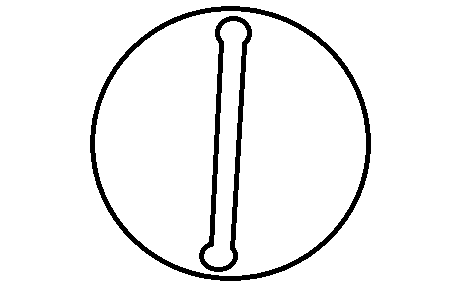
\includegraphics{sphereNotSimple}\par
Вырежем из северного и южного полюсов сферы кружочки, а затем разрежем её от одного кружочка до другого. Этим действием мы немного изменили промежутки принимаемых углами $\varphi$ и $\theta$ значений в сферических координатах, к которым мы и перейдем. Таким образом, теперь промежутки допустимых значений:
$$\frac{1}{n} \leq \varphi \leq 2 \pi - \frac{1}{n}$$
$$\frac{1}{n} \leq \theta \leq \pi - \frac{1}{n}$$
И теперь новая поверхность является простой.\par
\uline{Конус}:\par
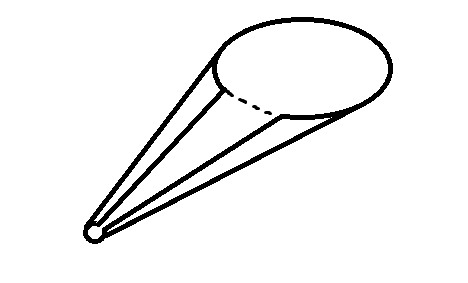
\includegraphics{coneNotSimple}\par
Вырежем вершину конуса и разрежем его по вертикали. Этим действием мы немного изменили промежутки допустимых значений для радиуса $r$ и угла $\varphi$ в цилиндрических координатах, к которым мы и перейдем. Таким образом, теперь промежутки допустимых значений:
$$\frac{1}{n} \leq r \leq n$$
$$\frac{1}{n} \leq \theta \leq 2 \pi - \frac{1}{n}$$
И теперь новая поверхность является простой.\par
\subsection{Функции, задающие одну и ту же поверхность}
Пусть даны $\Omega$ и $\Omega^{'}$, а так же соответствия $u=u(u^{'},v^{'}), v=v(u^{'},v^{'})$.\par
Кроме того, пусть якобиан $\begin{bmatrix} u_{u^{'}} & u_{v^{'}} \\ v_{u^{'}} & v_{v^{'}} \end{bmatrix}$ не равен 0 (то есть, существует обратная функция).\par
Это значит, что $\Omega$ отображается на $\Omega^{'}$ взаимно-однозначно.\par
В таком случае будем считать, что
$$\overrightarrow{r}(u,v) = \overrightarrow{r}(u(u^{'},v^{'}),v(u^{'},v^{'}))=\overrightarrow{\varrho}(u^{'},v^{'}) - \Sigma$$
(задают одну и ту же поверхность).
\subsection{Координатные кривые}
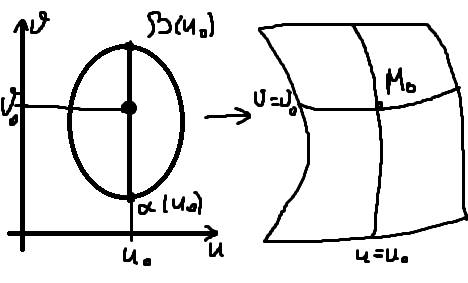
\includegraphics{coordCurves}\par
Зафиксируем одну из координат, например, $u=u_0$, и будем менять $v$ от $\alpha(u_0)$ до $\beta(u_0)$. Получим кривую $\overrightarrow{r}(u_0,v)$.\par
Аналогично, если зафиксировать $v=v_0$, то зададим кривую $\overrightarrow{r}(u,v_0)$.\par
Эти две кривые называются \textbf{координатными кривыми}.\par
\subsection{Нормаль}
Теперь рассмотрим $\overrightarrow{r}_u, \overrightarrow{r}_v$ - касательные к кривой.\par
Пусть $A = \begin{bmatrix}
   x_u & y_u & z_u \\
   x_v & y_v & z_v \\
\end{bmatrix}$, тогда если $rank A = 2$, то векторное произведение $\overrightarrow{r}_u \times \overrightarrow{r}_v \neq 0$.\par
Результат этого векторного произведения $\overrightarrow{r}_u \times \overrightarrow{r}_v = \overrightarrow{n}$ является вектором \textbf{нормали} к поверхности $\Sigma$.\par
Убедимся, что нормаль не зависит от параметризации кривой:\par
Дано взаимно-однозначное отображение $\Omega \iff \Omega^{'}$ и $\overrightarrow{r}(u,v) = \overrightarrow{\varrho}(u^{'},v^{'})$.\par
Посчитаем $\overrightarrow{\varrho}_{u^{'}} \times \overrightarrow{\varrho}_{v^{'}}$:\par
Вспомним, что $\overrightarrow{\varrho}(u^{'},v^{'}) = \overrightarrow{r}(u(u^{'},v^{'}),v(u^{'},v^{'}))$, это значит, что
$$\overrightarrow{\varrho}_{u^{'}} = \overrightarrow{r}_u \frac{\partial u}{\partial u^{'}} + \overrightarrow{r}_v \frac{\partial v}{\partial u^{'}},$$
$$\overrightarrow{\varrho}_{v^{'}} = \overrightarrow{r}_u \frac{\partial u}{\partial v^{'}} + \overrightarrow{r}_v \frac{\partial v}{\partial v^{'}}$$
Перемножим, учитывая, что векторное произведение коллинеарных векторов равно нулю:
$$\overrightarrow{\varrho}_{u^{'}} \times \overrightarrow{\varrho}_{v^{'}} = (\overrightarrow{r}_u \times \overrightarrow{r}_v) \frac{\partial u}{\partial u^{'}} \frac{\partial v}{\partial v^{'}} + (\overrightarrow{r}_v \times \overrightarrow{r}_u) \frac{\partial v}{\partial u^{'}} \frac{\partial u}{\partial v^{'}} = $$
$$ = (\overrightarrow{r}_u \times \overrightarrow{r}_v) (\frac{\partial u}{\partial u^{'}} \frac{\partial v}{\partial v^{'}}-\frac{\partial v}{\partial u^{'}} \frac{\partial u}{\partial v^{'}}) (\text{поменяли знак}) = (\overrightarrow{r}_u \times \overrightarrow{r}_v) \begin{bmatrix} u_{u^{'}} & u_{v^{'}} \\ v_{u^{'}} & v_{v^{'}} \end{bmatrix}$$

Но этот якобиан не равен нулю!\par
Это значит, что получили тот же вектор нормали, у которого могла измениться лишь длина или направление, что и требовалось доказать.\par
\subsection{Площадь поверхности}
Даны $\Omega, \overrightarrow{r}=\overrightarrow{r}(u,v)$.\par
Найдем дифференциал этого вектора:
$$d \overrightarrow{r} = \overrightarrow{r}_u du + \overrightarrow{r}_v dv$$
$$d \overrightarrow{r}^2 = |d \overrightarrow{r}|^2 = \overrightarrow{r}_u^2 du^2 + 2 \overrightarrow{r}_u \overrightarrow{r}_v dudv + \overrightarrow{r}_v^2 dv^2$$
Обозначим $E = \overrightarrow{r}_u^2, F = \overrightarrow{r}_u \overrightarrow{r}_v, G = \overrightarrow{r}_v^2$.\par
$d \overrightarrow{r}^2$ называется первой квадратичной формой поверхности и для неё справедливо свойство:\par
$d \overrightarrow{r}^2 > 0$ (положительно определена)ю\par
Для того, чтобы это выполнялось (для нашей формы $ax^2 + 2bxy + cy^2$), нужно:
$$\begin{cases} a > 0 \\ c > 0 \\ ac - b^2 > 0 \end{cases}$$
В нашем случае второго дифференциала вектора $\overrightarrow{r}$ это значит, что требуется выполнение следующих условий:
$$\begin{cases} E > 0 \\ G > 0 \\ EG - F^2 > 0 \end{cases}$$
Первые два условия очевидны, проверим третье:
$$| \overrightarrow{r}_u \times \overrightarrow{r}_v | = |\overrightarrow{r}_u| |\overrightarrow{r}_v| \sin \varphi \  (\varphi \neq 0)$$
$$\overrightarrow{r}_u \cdot \overrightarrow{r}_v = |\overrightarrow{r}_u| |\overrightarrow{r}_v| \cos \varphi$$
$$|\overrightarrow{r}_u \times \overrightarrow{r}_v|^2 + (\overrightarrow{r}_u \cdot \overrightarrow{r}_v)^2 = |\overrightarrow{r}_u|^2 |\overrightarrow{r}_v|^2$$

Заметим, что правая часть это $EG$, а второе слагаемое в левой части это $F^2$.\par
Тогда $|\overrightarrow{r}_u \times \overrightarrow{r}_v|^2 = EG-F^2 > 0$, так как $\overrightarrow{r}_u \times \overrightarrow{r}_v \neq 0$, что и требовалось доказать.\par
\uline{\textbf{Площадь поверхности}}\par\par
$S(\Sigma) = \iint_\Omega |\overrightarrow{r}_u \times \overrightarrow{r}_v| \ du dv$ - площадь поверхности.\par
Свойства площади:\par
1) Не зависит от параметризации.\par
Пусть дали две параметризации:
$$\overrightarrow{r}(u,v) = \overrightarrow{\varrho}(u^{'},v^{'})$$
$$S(\Sigma) = \iint_{\Omega^{'}} |\overrightarrow{\varrho}_{u^{'}} \times \overrightarrow{\varrho}_{v^{'}}| \ du^{'} dv^{'}$$
Вспомним, что $|\overrightarrow{\varrho}_{u^{'}} \times \overrightarrow{\varrho}_{v^{'}}| = |(\overrightarrow{r}_u \times \overrightarrow{r}_v)| \ |I(\frac{u,v}{u^{'},v^{'}})|$.\par
Подставим это в интеграл:
$$S(\Sigma) = \iint_{\Omega^{'}} |\overrightarrow{r}_u \times \overrightarrow{r}_v| \ |I| du^{'} dv^{'} = \iint_\Omega |\overrightarrow{r}_u \times \overrightarrow{r}_v| \ dudv$$
Получили то же самое.\par
2) Рассмотрим случай, когда сама поверхность - плоскость. Сможем ли по той же формуле посчитать площадь? Проверим это, площадь это $\iint_\Omega \ dudv$.\par
Теперь посчитаем $S(\Omega):$\par
$\Sigma$ задается при помощи $\overrightarrow{r} = (x,y,0)$.\par
Тогда $\overrightarrow{r}_x = (1,0,0)$\par
$\indent \overrightarrow{r}_y = (0,1,0)$.\par
А $\overrightarrow{r}_x \times \overrightarrow{r}_y = \begin{bmatrix} i & j & k \\ 1 & 0 & 0 \\ 0 & 1 & 0 \end{bmatrix} = \overrightarrow{k}, \Rightarrow |\overrightarrow{r}_x \times \overrightarrow{r}_y | = 1$.\par
Тогда $S(\Sigma) = \iint_\Omega |\overrightarrow{r}_x \times \overrightarrow{r}_y| \ du dv = \iint_\Omega du dv$, что и требовалось доказать.\par
3) Площадь аддитивна по отношению к поверхности. (Площадь поверхности, составленной из гладких кусков, равно сумме площадей).\par
4) $z = f(x,y)$.\par
$\overrightarrow{r} = (x,y,f(x,y))$.\par
$\overrightarrow{r}_x = (1,0,f_x)$.\par
$\overrightarrow{r}_y = (0,1,f_y)$.\par
$\overrightarrow{r}_x \times \overrightarrow{r}_y = \begin{bmatrix} i & j & k \\ 1 & 0 & f_x \\ 0 & 1 & f_y \end{bmatrix} = i (-f_x) - j f_y + \overrightarrow{k}$.
$$|\overrightarrow{r}_x \times \overrightarrow{r}_y| = \sqrt{EG - F} = \sqrt{f_x^2 + f_y^2 +1}$$
\uline{\textbf{ПРИМЕРЫ:}}\par
1) Посчитать площадь:
$$x^2 + y^2 + z^2 - R^2,$$
где $z \geq 0$.\par
Это половина сферы, которую вырезает цилиндр:
$$x^2 + y^2 = Rx, \Rightarrow x^2 - Rx + \frac{x^2}{4} + y^2 = (\frac{R}{2})^2, \Rightarrow (x-\frac{R}{2})^2 + y^2 = (\frac{R}{2})^2$$
Это выглядит так:\par
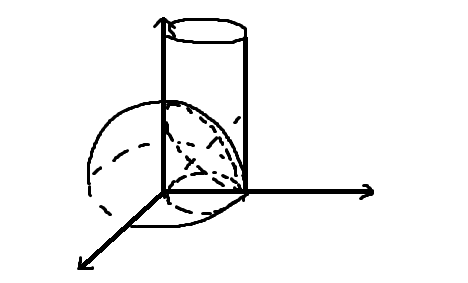
\includegraphics{halfSphereAndCylindr1}\par
Перейдем в сферические координаты:\par
$\begin{cases} x = R\cos\varphi \sin\theta \\ y = R \sin \varphi \sin \theta \\ z = R \cos \theta \end{cases}$.\par
Зададим поверхность:
$$\overrightarrow{r} = (R\cos\varphi \sin\theta, R\sin\varphi \sin\theta, R\cos\theta)$$

Посчитаем частные производные по $\varphi$ и $\theta$:\par
$\overrightarrow{r}_\varphi = (-R \sin \varphi \sin \theta, R\cos\varphi \sin \theta, 0)$\par
$\overrightarrow{r}_\theta = (R\cos\varphi \cos\theta, R\sin\varphi \cos\theta, -R\sin\theta)$\par
Теперь посчитаем $E, F, G$:\par
$E = \overrightarrow{r}_\varphi^2 = R^2 \sin^2 \varphi \sin^2 \theta + R^2 \cos^2 \varphi \sin^2 \theta = R^2 \sin^2 \theta$.\par
$F = \overrightarrow{r}_\theta^2 = R^2 \cos^2 \varphi \cos^2 \theta + R^2 \sin^2 \varphi \cos^2 \theta + R^2 \sin^2 \theta = R^2$.\par
$F = 0$ (если раскрыть скобки, то и правда получится 0).\par
$\sqrt{EG-F^2} = R^2 \sin\theta$.\par
Тогда $S(\Sigma) = \iint_\Omega R^2 \sin\theta \ d\varphi d\theta = 2 R^2 \int_0^{\frac{\pi}{2}} d\varphi \int_0^? \sin\theta \ d\theta$.\par
Осталось вычислить верхний предел интегрирования для $\theta$, для этого нужно подставить сферические координаты в уравнение цилиндра:\par
$R^2 \cos^2 \varphi \sin^2 \theta + R^2 \sin^2 \varphi \sin^2\theta = R^2 \cos\varphi \sin\theta$.\par
Отсюда либо $\sin\theta = 0$, либо $\sin\theta = \cos\varphi$.\par
Первое нас не интересует, а вот второе можно решить и получить ответ:\par
$\theta = \frac{\pi}{2} - \varphi$.\par
Тогда $S(\Sigma) = \iint_\Omega R^2 \sin\theta \ d\varphi d\theta = 2 R^2 \int_0^{\frac{\pi}{2}} d\varphi \int_0^{\frac{\pi}{2} - \varphi} \sin\theta \ d\theta = R^2(\pi - 2)$.\par
2) Посчитать площадь поверхности:\par
$z = x^2 + y^2$. Этот параболоид бесконечен, поэтому чтобы было, что считать, вырежем из него кусок $x^2 + y^2 = R^2$ и найдем площадь.\par
Вот как это выглядит:\par
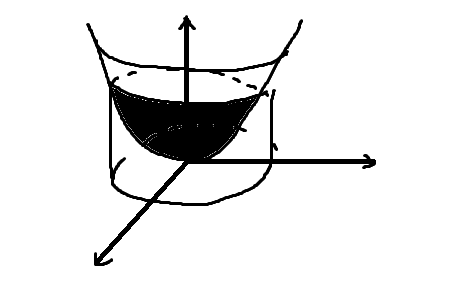
\includegraphics{paraboloidAndCylindr1}\par
Для этого перейдем к цилиндрическим координатам:\par
$\begin{cases} x=\varrho \cos \varphi \\ y = \varrho \sin \varphi \\ z = \varrho^2 \end{cases}$.\par
Зададим поверхность:\par
$\overrightarrow{r} = (\varrho\cos\varphi, \varrho\sin\varphi, \varrho^2)$.\par
Посчитаем частные производные по $\varrho$ и $\varphi$.\par
$\overrightarrow{r}_\varrho = (\cos\varphi, \sin\varphi, 2\varrho)$.\par
$\overrightarrow{r}_\varphi = (-\varrho\sin\varphi, \varrho\cos\varphi, 0)$.\par
Теперь посчитаем $E, F, G$:\par
$E = \overrightarrow{r}_\varrho^2 = 1 + 4 \varrho^2$.\par\par
$F = \overrightarrow{r}_\varphi^2 = \varrho^2$.\par
$F = 0$ (если раскрыть скобки, то и правда получится 0).\par
$\sqrt{EG-F^2} = \varrho\sqrt{1+4\varrho^2}$.
$$S(\Sigma)=\iint_\Omega \varrho\sqrt{1+4\varrho^2} \ d\varrho d\varphi = \int_0^{2\pi} d\varphi \int_0^R \varrho\sqrt{1+4\varrho^2} \ d\varrho$$
\uline{Важная информация про почти простые поверхности:}\par
\uline{Утверждение:} если $\Sigma$ - почти простая, а $\Omega_n$ - искомая исчерпывающая последовательность, то:
$$S(\Sigma) = \iint_\Omega |\overrightarrow{r}_u \times \overrightarrow{r}_v| \ dudv = \lim_{n\to\infty} \iint_{\Omega_n} |\overrightarrow{r}_u \times \overrightarrow{r}_v| \ dudv$$
\section{Поверхностные интегралы}
\subsection{Поверхностный интеграл первого рода}
Пусть $\Sigma$ - простая и гладкая поверхность. Дана $F(x,y,z)$ - непрерывная функция, определенная на $\Sigma$.\par
Поверхностным интегралом $\Romannum{1}$ рода от функции $F$ по поверхности $\Sigma$ называется:
$$\iint_\Omega F(x(u,v),y(u,v),z(u,v)) | \overrightarrow{r}_u \times \overrightarrow{r}_v| \ dudv = \iint_\Sigma F(x,y,z) ds (d\sigma)$$
\uline{Свойства поверхностного интеграла $\Romannum{1}$ рода:}\par
1) Не зависит от параметризации поверхности (доказывается так же, как независимость площади поверхности от параметризации).\par
2) Аддитивность и линейность.\par
3) Можно дать физическую интерпретацию:\par
Если $F(x,y,z) \geq 0$, и это плотность слоя, ''намазанного'' на поверхность, то $\iint F d\sigma$ - масса слоя.\par
\textbf{Вместо $d\sigma$ можно написать $\sqrt{EG-F^2} \ dudv$}.\par
\subsection{Поверхностный интеграл второго рода}
Пусть $\Sigma$ - двусторонняя (бывают односторонние поверхности, например, лист Мёбиуса и бутылка Клейна (Кляйна)). Выберем сторону (это означает, выберем, куда ''смотрит'' нормаль).\par
У нас есть поверхностный интеграл $\iint_\Sigma (\overrightarrow{F}, \overrightarrow{n}_0) \ d\sigma$, \par
где $\overrightarrow{F} = (P(x,y,z),Q(x,y,z),R(x,y,z))$.\par
Если поменять сторону, то поменяется знак за счёт смены направления вектора нормали на противоположное.\par
Отсюда вытекает свойство:
$$\iint_\Sigma (\overrightarrow{F}, \overrightarrow{n}_0) \ d\sigma = -\iint_\Sigma (\overrightarrow{F}, \overrightarrow{n}_0^{-}) \ d\sigma$$
\subsection{Как считать поверхностный интеграл второго рода}
Рассмотрим $(\overrightarrow{F}, \overrightarrow{n}_0) = \overrightarrow{F} \frac{\overrightarrow{r}_u \times \overrightarrow{r}_v}{|\overrightarrow{r}_u \times \overrightarrow{r}_v|} \ |\overrightarrow{r}_u \times \overrightarrow{r}_v| \ dudv = (\overrightarrow{F} \cdot \overrightarrow{r}_u \cdot \overrightarrow{r}_v) \ dudv$ (смешанное произведение).\par
Посчитаем его:
$$\begin{bmatrix} R & Q & R \\ x_u & y_u & z_u \\ x_v & y_v & z_v \end{bmatrix} \ dudv =$$
$$= (P \frac{\partial (y,z)}{\partial(u,v)} + Q \frac{\partial (z,x)}{\partial(u,v)}\text{(поменяли знак)} + R\frac{\partial (x,y)}{\partial(u,v)}) \ dudv$$
Рассмотрим $PI (\frac{y,z}{u,v}) \ du dv$:\par
Если угол между вектором нормали и осью $x$ острый, то $I > 0$, иначе $I < 0$.\par
Тогда для острого угла $\iint PI \ du dv = \iint_{D_{yz}} P (x(y,z),y,z) \ dydz$.\par
А для тупого угла $\iint PI \ du dv = - \iint_{D_{yz}} P (x(y,z),y,z) \ dydz$.\par
Аналогично и другие слагаемые, тогда запишем сумму:\par
$P \frac{\partial (y,z)}{\partial(u,v)}\ dudv + Q \frac{\partial (z,x)}{\partial(u,v)}\ dudv + R\frac{\partial (x,y)}{\partial(u,v)} \ dudv = P\ dydz + Q\ dzdx + R \ dxdy$.\par
Тогда
$$\iint_\Sigma (\overrightarrow{F}, \overrightarrow{n}_0) \ d\sigma = \iint_\Sigma P \ dydz + Q \ dzdx + R \ dxdy$$
\uline{\textbf{ПРИМЕР:}}\par
Дан $\iint_\Sigma x \ dydz$, и вырезан прямоугольник $z + y - x = 1$, верхняя сторона.\par
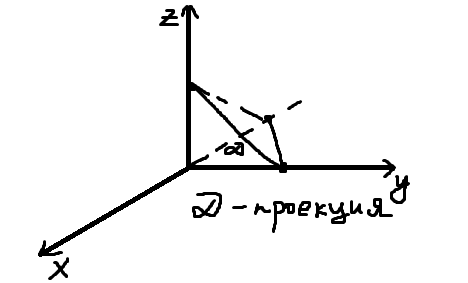
\includegraphics{triangleCut1}
Посчитаем:\par
$\iint_\Sigma x \ dydz = - \iint (z+y-1)\ dydz$ (так как угол между нормалью и отсутствующей осью (в данном случае ось $x$) тупой).
$$- \iint (z+y-1)\ dydz = - \int_0^1 dy \int_0^{1-y}(z+(y-1))\ dz = \frac{1}{6}$$
\section{Теория поля}
$\Omega \subset R^3$.\par
\Romannum{1}. Скалярное поле.\par
Если $\forall M \in \Omega \ \exists f(M)$ - число, тогда у нас на области $\Omega$ задано скалярное поле $f(M) = f(x,y,z)$.\par
\uline{Дифференцируемость.}\par
\uline{Определение:} будем называть $f(M)$ дифференцируемым в точке $M_0$, если существует такой вектор $\overrightarrow{c}$, что
$${\bigtriangleup f}(M_0) = {\bigtriangleup \overrightarrow{r}} \cdot \overrightarrow{c} + o(||\overrightarrow{MM_0}||)$$
$$\overrightarrow{c} = grad f(M_0) = (\frac{\partial f(M_0)}{\partial x}, \frac{\partial f(M_0)}{\partial y}, \frac{\partial f(M_0)}{\partial z})$$
Гуманитарии могут делать так:\par
$\sin x + \cos x = (\sin+\cos)x$.\par
Мы сделаем так для градиента, но осознанно и опираясь на законы:
$$(\frac{\partial f}{\partial x},\frac{\partial f}{\partial y}, \frac{\partial f}{\partial z}) = (\frac{\partial}{\partial x},\frac{\partial}{\partial y},\frac{\partial}{\partial z})f$$
Обозначим теперь $(\frac{\partial}{\partial x},\frac{\partial}{\partial y},\frac{\partial}{\partial z})$ за $\nabla$ (произносится ''набла'').\par
Это символический вектор, его координаты это вроде числа, но на самом деле, эта набла - целиком оператор и применяется к чему-то.\par
Тогда $(\frac{\partial f}{\partial x},\frac{\partial f}{\partial y}, \frac{\partial f}{\partial z}) = {\nabla f}$.\par
$\overrightarrow{c} = {\nabla f}$, тогда
$${\bigtriangleup f} = {\bigtriangleup \overrightarrow{r}} \cdot {\nabla f} = ({\bigtriangleup \overrightarrow{r}} \cdot {\nabla})f + o(||\overrightarrow{MM_0}||)$$
\uline{Производная по направлению.}
$$\frac{\partial f (M_0)}{\partial l} = \lim{t\to 0} \frac{f(M_0+t\overrightarrow{l_0})-f(M_0)}{\partial t}$$
Здесь $t > 0$, а $\overrightarrow{l_0}$ - орт направления.\par
Заметим, что числитель - приращение, так что можно переписать в виде:
$$\frac{\partial f (M_0)}{\partial l} = \lim{t\to 0} \frac{(t \overrightarrow{l_0} \cdot \nabla + o(t)}{\partial t} = (\overrightarrow{l_0} \cdot \nabla)f$$
\Romannum{2}. Векторное поле.\par
Если $\forall M \in \Omega \ \exists \overrightarrow{a}(M) = (P(x,y,z),Q(x,y,z),R(x,y,z))$, тогда на области $\Omega$ задано векторное поле $\overrightarrow{a}(M) = (P(x,y,z),Q(x,y,z),R(x,y,z))$.\par
\uline{Дифференцируемость.}\par
\uline{Определение:} будем называть $\overrightarrow{a}(M)$ дифференцируемым в точке $M_0$, если его приращение можно представить в виде:
$${\bigtriangleup \overrightarrow{a}(M)} = \overrightarrow{a}(M) - \overrightarrow{a}(M_0) = L(\overrightarrow{r})+o(||\overrightarrow{r}||)$$
Тогда
$${\bigtriangleup \overrightarrow{a}(M)} = ({\bigtriangleup \overrightarrow{r}} \cdot \nabla)\overrightarrow{a} + o(||\overrightarrow{r}||)$$
\uline{Производная по направлению.}\par
$\frac{\partial f}{\partial l} = (\overrightarrow{l_0} \cdot \nabla)f$ - для скалярного поля. В случае векторного поля:
$$\frac{\partial \overrightarrow{a}}{\partial l} = (\overrightarrow{l_0} \cdot \nabla)\overrightarrow{a}$$
\uline{\textbf{ПРИМЕР:}}\par
$\overrightarrow{a} = y \overrightarrow{i} + (xy + yz)\overrightarrow{j} + xyz \overrightarrow{k}$\par
$\overrightarrow{l} = (1,1,1), \overrightarrow{l_0} = (\frac{1}{\sqrt{3}},\frac{1}{\sqrt{3}},\frac{1}{\sqrt{3}})$\par
$\frac{\partial \overrightarrow{a}}{\partial l} = (\overrightarrow{l_0} \cdot \nabla)\overrightarrow{a}$\par
1) $(\overrightarrow{l_0} \cdot \nabla)\overrightarrow{a} = \frac{1}{\sqrt{3}} \frac{\partial}{\partial x} + \frac{1}{\sqrt{3}} \frac{\partial}{\partial y} + \frac{1}{\sqrt{3}} \frac{\partial}{\partial z}$, и все это нужно применить к вектору $\overrightarrow{a}$.\par
2) $(\overrightarrow{l_0} \cdot \nabla)\overrightarrow{a}$ - рассмотрим результат покоординатно:\par
$(\overrightarrow{l_0} \cdot \nabla)a_x = (\frac{1}{\sqrt{3}} \frac{\partial}{\partial x},\frac{1}{\sqrt{3}} \frac{\partial}{\partial y},\frac{1}{\sqrt{3}} \frac{\partial}{\partial z})y = \frac{1}{\sqrt{3}}$\par
$(\overrightarrow{l_0} \cdot \nabla)a_y = (\frac{1}{\sqrt{3}} \frac{\partial}{\partial x},\frac{1}{\sqrt{3}} \frac{\partial}{\partial y},\frac{1}{\sqrt{3}} \frac{\partial}{\partial z})(xy+yz) = \frac{2y+x+z}{\sqrt{3}}$\par
$(\overrightarrow{l_0} \cdot \nabla)a_z = (\frac{1}{\sqrt{3}} \frac{\partial}{\partial x},\frac{1}{\sqrt{3}} \frac{\partial}{\partial y},\frac{1}{\sqrt{3}} \frac{\partial}{\partial z})(xy) = \frac{yz+xz+xy}{\sqrt{3}}$\par
Тогда\par
$(\overrightarrow{l_0} \cdot \nabla)\overrightarrow{a} = \frac{1}{\sqrt{3}}\overrightarrow{i} + \frac{2y+x+z}{\sqrt{3}}\overrightarrow{j} + \frac{yz+xz+xy}{\sqrt{3}}\overrightarrow{k}$.\par
\uline{Введем понятия:}\par
Пусть дано поле $\overrightarrow{a} = \overrightarrow{a}(M) = (P,Q,R)$.\par
\uline{Определение:} \textbf{дивергенция} поля:
$$div\overrightarrow{a} = \frac{\partial P}{\partial x} + \frac{\partial Q}{\partial y} + \frac{\partial R}{\partial z}$$
\uline{Определение:} \textbf{ротор} векторного поля:
$$rot\overrightarrow{a} = det \begin{bmatrix} i & j & k \\ \frac{\partial}{\partial x} & \frac{\partial}{\partial y} & \frac{\partial}{\partial z} \\ P & Q & R \end{bmatrix} = \overrightarrow{i} (\frac{\partial R}{\partial y} - \frac{\partial Q}{\partial z}) + \overrightarrow{j}(\frac{\partial P}{\partial z} - \frac{\partial R}{\partial x}) + \overrightarrow{k}(\frac{\partial Q}{\partial x} - \frac{\partial P}{\partial y})$$
Упростим формулы для $div$ и $rot$:\par
$div \overrightarrow{a} = (\nabla \cdot \overrightarrow{a})$ (скалярное произведение).\par
$rot \overrightarrow{a} = (\nabla \times \overrightarrow{a})$ (векторное произведение).\par
\uline{\textbf{Действия с $\nabla$}}:\par
1) $$\nabla(c_1 f_1 + c_2 f_2) = c_1 {\nabla f_1} + c_2 {\nabla f_2}$$
2) Посчитаем $\nabla(f_1 f_2)$:
$$\frac{\partial}{\partial x}(f_1 f_2) = \frac{\partial f_1}{\partial x} f_2 + \frac{\partial f_2}{\partial x} f_1$$
$$\frac{\partial}{\partial y}(f_1 f_2) = \frac{\partial f_1}{\partial y} f_2 + \frac{\partial f_2}{\partial y} f_1$$
$$\frac{\partial}{\partial z}(f_1 f_2) = \frac{\partial f_1}{\partial z} f_2 + \frac{\partial f_2}{\partial z} f_1$$
Будем иметь ввиду, что $\nabla$ действует на поле, когда пишем следующим образом:
$$\nabla(\overset{\downarrow}{f_1} f_2)$$
Здесь $\nabla$ действует на поле $f_1$.\par
Тогда $\nabla(f_1 f_2) = \nabla(\overset{\downarrow}{f_1} f_2) + \nabla(f_1 \overset{\downarrow}{f_2}) = f_1 {\nabla f_2} + f_2 {\nabla f_1}$.\par
3) Посчитаем $\nabla(\overrightarrow{a_1} \times \overrightarrow{a_2})$:\par
Формально это смешанное произведение, тогда
$$\nabla(\overrightarrow{a_1} \times \overrightarrow{a_2}) = \nabla(\overset{\downarrow}{\overrightarrow{a_1}} \times \overrightarrow{a_2}) + \nabla(\overrightarrow{a_1} \times \overset{\downarrow}{\overrightarrow{a_2}}) = \overrightarrow{a_2}(\nabla \times \overrightarrow{a_1})-\overrightarrow{a_1}(\nabla \times \overrightarrow{a_2})$$
4) $grad \ f = {\nabla f}$\par
5) $grad \ (f_1 f_2) = f_1 grad \ f_2 + f_2 grad \ f_1$\par
6) $div \overrightarrow{a} = \nabla \cdot \overrightarrow{a}$\par
7) $rot \overrightarrow{a} = \nabla \times \overrightarrow{a}$\par
8) $div (f \cdot \overrightarrow{a}) = \nabla(f \cdot \overrightarrow{a}) = \nabla(\overset{\downarrow}{f} \cdot \overrightarrow{a}) + \nabla(f \cdot \overset{\downarrow}{\overrightarrow{a}}) =\overrightarrow{a} \nabla f + f \nabla \overrightarrow{a} = \overrightarrow{a} grad \ f + f div \overrightarrow{a}$\par
9) $div (\overrightarrow{a_1} \times \overrightarrow{a_2}) = \nabla(\overrightarrow{a_1} \times \overrightarrow{a_2}) = \nabla(\overset{\downarrow}{\overrightarrow{a_1}} \times \overrightarrow{a_2}) + \nabla(\overrightarrow{a_1} \times \overset{\downarrow}{\overrightarrow{a_2}}) = \overrightarrow{a_2}(\nabla \times \overrightarrow{a_1}) - \overrightarrow{a_1} (\nabla \times \overrightarrow{a_2}) = \overrightarrow{a_2} rot \overrightarrow{a_1} - \overrightarrow{a_1} rot \overrightarrow{a_2}$\par
10) $rot(f\overrightarrow{a}) = \nabla \times (f\overrightarrow{a}) = \nabla \times (\overset{\downarrow}{f}\overrightarrow{a}) + \nabla \times (f\overset{\downarrow}{\overrightarrow{a}}) = ({\nabla f}) \times \overrightarrow{a} + f(\nabla \times \overrightarrow{a})  = grad \ f \times \overrightarrow{a} + f \ rot \overrightarrow{a}$\par
11) $rot(\overrightarrow{a_1} \times \overrightarrow{a_2}) = \nabla (\overrightarrow{a_1} \times \overrightarrow{a_2}) = \nabla \overset{\downarrow}{\overrightarrow{a_1}} \times \overrightarrow{a_2} + \nabla \overrightarrow{a_1} \times \overset{\downarrow}{\overrightarrow{a_2}} = (\overrightarrow{a_2} \nabla)\overrightarrow{a_1} - \overrightarrow{a_2}(\nabla \overrightarrow{a_1}) + \overrightarrow{a_1}(\nabla  \overrightarrow{a_2}) - (\overrightarrow{a_1} \nabla)\overrightarrow{a_2} = (\overrightarrow{a_2} \nabla)\overrightarrow{a_1} - \overrightarrow{a_2} div \overrightarrow{a_1} + \overrightarrow{a_1} div \overrightarrow{a_2} - (\overrightarrow{a_1} \nabla)\overrightarrow{a_2}$\par
12) $div (grad \ f) = \nabla \cdot ({\nabla f}) = \frac{\partial^2 f}{\partial x^2} + \frac{\partial^2 f}{\partial y^2} + \frac{\partial^2 f}{\partial z^2} = (\frac{\partial}{\partial x^2} + \frac{\partial}{\partial y^2} + \frac{\partial}{\partial z^2})f =\\= \nabla^2 f = \bigtriangleup f$.\par
$\bigtriangleup$ - оператор Лапласа, $\bigtriangleup = \nabla^2$.\par
13) $div (rot \overrightarrow{a}) = \nabla \cdot (\nabla \times \overrightarrow{a}) = 0$.\par
14) $rot (grad \ f) = \nabla \times (\nabla \cdot f) = 0$.\par
\textbf{\uline{Экскурс в физику - физический смысл ротора}}\par
Пусть дали твердое тело, оно вращается вокруг какой то оси, пусть по часовой стрелке:\par
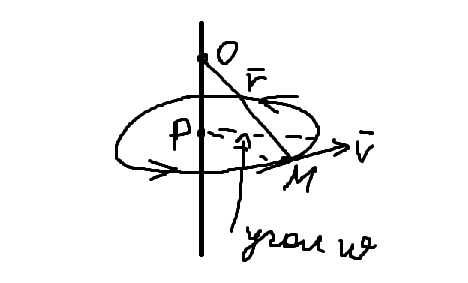
\includegraphics{rotorPhysicDefinition}\par
$|\overrightarrow{v}| = PM$(радиус)$\cdot \omega$.\par
Вектор $\overrightarrow{\omega} \times \overrightarrow{r}$ параллелен $\overrightarrow{v}$ (1)\par
$|\overrightarrow{v}| = \omega \cdot |\overrightarrow{r}| \sin \varphi = |\overrightarrow{\omega}| \ |\overrightarrow{r}| \sin (\pi - \varphi)$ (2)\par
Из (1) и (2) следует, что $\overrightarrow{v} = \overrightarrow{\omega} \times \overrightarrow{r}$.\par
Посчитаем $rot (\overrightarrow{v})$:\par
$rot(\overrightarrow{v})=rot(\overrightarrow{\omega} \times \overrightarrow{r}) = \overrightarrow{\omega} div \overrightarrow{r} - \overrightarrow{r} div \overrightarrow{\omega} + (\overrightarrow{r} \nabla) \overrightarrow{\omega} - (\overrightarrow{\omega} \nabla) \overrightarrow{r}$.\par
$\overrightarrow{\omega}$ зависит только от времени, следовательно, везде, где дифференцируем $\overrightarrow{\omega}$, будут нули:\par
$div \overrightarrow{\omega} = 0, (\overrightarrow{r} \nabla) \overrightarrow{\omega} = 0$.\par
Тогда $rot \overrightarrow{v} = \overrightarrow{\omega} div \overrightarrow{r} - (\overrightarrow{\omega} \nabla)\overrightarrow{r} = 3\overrightarrow{\omega} - \overrightarrow{\omega} = 2\overrightarrow{\omega}$.\par
Таким образом, физический смысл ротора: удвоенная мгновенная угловая скорость, отсюда и его названия (ротор, вихрь).\par
\section{Интегральные характеристики векторного поля}
Дано векторное поле $\overrightarrow{a} = \overrightarrow{a}(M)$ в $\Omega$, а так же $l$ - простой кусочно-гладкий замкнутый контур из $\Omega$.\par
\subsection{Циркуляция}
\uline{Определение:} \textbf{циркуляцией} векторного поля по замкнутому контуру $l$ называется следующий интеграл второго рода:
$$\text{Ц} = \int_l \overrightarrow{a} d\overrightarrow{r} = \int_l Pdx + Qdy + Rdz$$
\subsection{Поток}
Дана поверхность $\Sigma$.\par
\uline{Определение:} \textbf{потоком} векторного поля по поверхности $\Sigma$ называется следующий интеграл второго рода:
$$\prod = \iint_{\Sigma} \overrightarrow{a} \overrightarrow{n_0} ds$$
Приведем к привычному виду:
$$\prod = \iint_{\Sigma} \overrightarrow{a} \overrightarrow{n_0} ds = \iint_{\Sigma} Pdydz + Qdzdx + Rdxdy$$
\textbf{Физический смысл потока}\par
Пусть есть $\overrightarrow{a} = \overrightarrow{v}$ - поле скоростей. Жидкость движется по какому-то пути, а затем мы ставим на этом пути решетку:\par
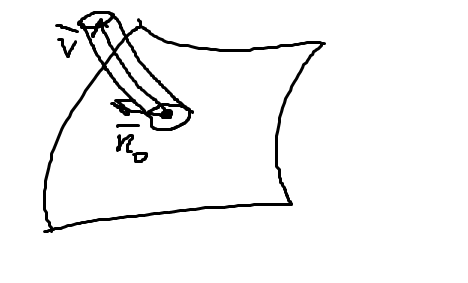
\includegraphics{currentPhysicDefinition}\par
И сколько жидкости проходит через решетку за единицу времени?\par
Возьмем в нашей решетке маленький кусок, из-за пренебрежимо малой величины можем считать его плоским. Тогда за единицу времени жидкость займет объем цилиндра с площадью основания, равной площади куска, и высотой, равной проекции $\overrightarrow{v}$ на ось вращения.\par
Посчитаем этот объем:
$$V_{\text{Ц}} = S \cdot |\overrightarrow{v}_{\text{пр.} \overrightarrow{n_0}}| = ds \overrightarrow{a} \overrightarrow{n_0} = d\prod$$
И поток будет равен приближенной сумме объемов по всем кусочкам, то есть интегралу.\par
\section{Теорема Гаусса-Остроградского}
Пусть есть ограниченная область $\Omega \subset R^3$\par
Граница этой области - $\partial \Omega$ - кусочно-гладкая.\par
$\overrightarrow{n}$ - внешняя нормаль.\par
$\overrightarrow{a} = \overrightarrow{a} (M), M \in \overrightarrow{\Omega}, \overrightarrow{a}$ непрерывно дифференцируемо в каждой точке.\par
\uline{Утверждение (теорема Остроградского-Гаусса):} выполняется равенство:
$$\iint_{\partial\Omega} \overrightarrow{a} \overrightarrow{n_0} ds = \iiint_{\Omega} div \overrightarrow{a} dxdydz$$
\uwave{Доказательство}:\par
Предположим, что $\Omega$ односвязна и элементарна по всем координатам.\par
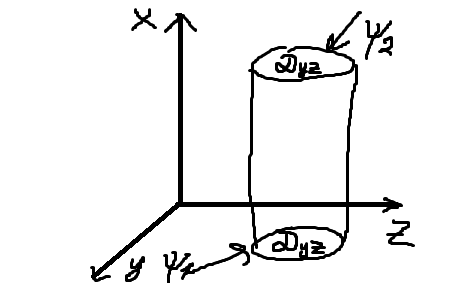
\includegraphics{ostrogradGaussProof}\par
Посчитаем одно из слагаемых, например, интеграл по $\frac{\partial P}{\partial x}$:\par
$\iiint_\Omega \frac{\partial P}{\partial x} dxdydz = \iint_{D_{yz}} dydz \int_{\psi_1(y,z)}^{\psi_2(y,z)} \frac{\partial P}{\partial x} =\\= \iint_{D_{yz}} P(\psi_2(y,z),y,z)dydz-\iint_{D_{yz}} P(\psi_1(y,z),y,z)dydz =\\= \iint_{\Sigma_1} P(x,y,z) dydz + \iint_{\Sigma_2} P(x,y,z) dydz + 0$ (интеграл по боковой поверхности равен нулю).\par
Здесь $\Sigma_1$ образована функцией $x = \psi_1(y,z)$, $\Sigma_2$ образована функцией $x = \psi_2(y,z)$.\par
Тогда эта сумма - интеграл по всей границе (три слагаемых это интеграл по верхней части, нижней части и боковой поверхности), а значит, она равна
$$\iint_{\partial \Omega} P(x,y,z) dydz$$
Аналогично доказывается для $Q$ и для $R$.\par
\subsection{Следствие из теоремы Остроградского-Гаусса}
Возьмем непрерывно дифференцируемое векторное поле $\overrightarrow{a} = (P,Q,R)$ в открытой области $\Omega$.\par
Возьмем из этой области точку $M_0$ и окружим ее сферой $S(M_0)$.\par
Обозначим за $V(M_0)$ шар, ограниченный сферой $S$, $V \subset \Omega$.\par
Запишем для сферы и шара формулу Остроградского-Гаусса:
$$\iint_{S(M_0)} \overrightarrow{a} \overrightarrow{n_0} ds =\iiint_{V(M_0)} div \overrightarrow{a} dV = I$$
\uline{Утверждение:} для какой-то точки $\overset{\sim}{M} \in V(M_0)$ выполняется равенство:
$$I = div \overrightarrow{a} (\overset{\sim}{M}) \cdot \textbf{V}$$
$\textbf{V}$ - объем шара. Отсюда выразим дивергенцию:
$$div \overrightarrow{a} (\overset{\sim}{M}) = \frac{\iint_{S(M_0)} \overrightarrow{a} \overrightarrow{n_0} ds}{\textbf{V}}$$
Полученную формулу принято называть средней плотностью источников (или стоков).\par
Какой в этом смысл:\par
Представим, что где-то через шар протекает жидкость. В нормальной ситуации вытекает жидкости ровно столько, сколько втекает, дивергенция равна нулю. Но если внутри шара есть источник/сток, тогда втекать будет меньше/больше, чем вытекать. Именно это и регулирует числитель в формуле дивергенции, полученной выше.\par
\section{Теорема Стокса}
Дано:\par
Простая и гладкая ($\overrightarrow{r}_u \times \overrightarrow{r}_v \neq \overrightarrow{0}$) поверхность $\overrightarrow{r} = \overrightarrow{r} (u,v) = \Sigma$.\par
Плоскость $\Omega \subset R^2 \to R^3, (u,v) \in \Omega, \Omega$ - ограничена.\par
$\partial \Omega = \{ u(t), v(t) \}, \alpha \leq t \leq \beta$.\par
$\overrightarrow{r}(t) = \overrightarrow{r}(u(t),v(t))$ - граница поверхности, $\partial \Sigma$.\par
Теорема (Стокса):\par
\uline{Утверждение:} имеет место формула:
$$\int_{\partial \Sigma} \overrightarrow{a} d \overrightarrow{r} = \iint_{\Sigma} rot \overrightarrow{a} \cdot \overrightarrow{n_0} ds$$
\uwave{Доказательство}:\par
1) Сведем $\int_{\partial \Sigma} \overrightarrow{a} d \overrightarrow{r}$ к интегралу по контуру $\partial \Omega$:
$$\int_{\partial \Sigma} \overrightarrow{a} d \overrightarrow{r} = \int_{\alpha}^{\beta} \overrightarrow{a} (\overrightarrow{r}(u(t),v(t))) \cdot (\overrightarrow{r}_u u_t dt + \overrightarrow{r}_v v_t dt)=$$
$$= \int_{\partial \Omega} \overrightarrow{a} (\overrightarrow{r}(u,v)) (\overrightarrow{r}_u du + \overrightarrow{r}_v dv) = I_1$$
2) Сведем $\iint_{\Sigma} rot \overrightarrow{a} \cdot \overrightarrow{n_0} ds$ к интегралу по области $\Omega$:
$$\iint_{\Sigma} rot \overrightarrow{a} \cdot \overrightarrow{n_0} ds = \iint_{\Omega} rot \overrightarrow{a} \cdot (\frac{(\overrightarrow{r}_u \times \overrightarrow{r}_v)}{|\overrightarrow{r}_u \times \overrightarrow{r}_v|} |\overrightarrow{r}_u \times \overrightarrow{r}_v|) du dv =$$
$$= \iint_{\Omega} rot \overrightarrow{a} \cdot (\overrightarrow{r}_u \times \overrightarrow{r}_v) du dv = I_2$$
Рассмотрим подынтегральное выражение, оно представляет собой смешанное произведение, попробуем представить его в виде $\frac{\partial Q}{\partial x} - \frac{\partial P}{\partial y}$, чтобы применить формулу Грина в обратную сторону:
$$rot \overrightarrow{a} \cdot (\overrightarrow{r}_u \times \overrightarrow{r}_v) = rot \overrightarrow{a} \cdot \overrightarrow{r}_u \cdot \overrightarrow{r}_v = \overrightarrow{r}_u \cdot \overrightarrow{r}_v \times (\nabla \times \overrightarrow{a}) =$$
$$=\overrightarrow{r}_u \cdot \nabla (\overrightarrow{r}_v \cdot \overset{\downarrow}{\overrightarrow{a}}) - \overrightarrow{r}_u (\overrightarrow{r}_v \cdot \nabla) \overrightarrow{a} = (\overrightarrow{r}_u \cdot \nabla)(\overrightarrow{r}_v \cdot \overset{\downarrow}{\overrightarrow{a}}) - \overrightarrow{r}_u(\overrightarrow{r}_v \cdot \nabla) \overrightarrow{a}=$$
$$= \overrightarrow{r}_v (\overrightarrow{r}_u \cdot \nabla) \overrightarrow{a} - \overrightarrow{r}_u (\overrightarrow{r}_v \cdot \nabla) \overrightarrow{a} = \overrightarrow{r}_v (x_u \frac{\partial \overrightarrow{a}}{\partial x} + y_u \frac{\partial \overrightarrow{a}}{\partial y} + z_u \frac{\partial \overrightarrow{a}}{\partial z}) -$$
$$- \overrightarrow{r}_u (x_v \frac{\partial \overrightarrow{a}}{\partial x} + y_v \frac{\partial \overrightarrow{a}}{\partial y} + z_v \frac{\partial \overrightarrow{a}}{\partial z}) =$$
$$= \overrightarrow{r}_v \overrightarrow{a}_u - \overrightarrow{r}_u \overrightarrow{a}_v = \overrightarrow{r}_v \overrightarrow{a}_u - \overrightarrow{r}_u \overrightarrow{a}_v + \overrightarrow{r}_{uv} \overrightarrow{a}_{uv} - \overrightarrow{r}_{uv} \overrightarrow{a}_{uv} =$$
$$ \frac{\partial}{\partial u}(\overrightarrow{a} \cdot \overrightarrow{r}_v) - \frac{\partial}{\partial v} (\overrightarrow{a} \cdot \overrightarrow{r}_u)$$
Получили как раз, что хотели, осталось подставить в $I_2$:
$$I_2 = \iint_{\Omega} (\frac{\partial}{\partial u}(\overrightarrow{a} \cdot \overrightarrow{r}_v) - \frac{\partial}{\partial v} (\overrightarrow{a} \cdot \overrightarrow{r}_u)) du dv$$
Тогда по формуле Грина для этого интеграла:
$$I_2 = \int_{\partial \Omega} \overrightarrow{a} \overrightarrow{r}_u du + \overrightarrow{a} \overrightarrow{r}_v dv = I_1$$
Таким образом, получили тот же интеграл, следовательно, формула верна и теорема доказана.\par
\subsection{Следствие из теоремы Стокса}
Дан интеграл $I = \int_{AB} Pdx + Qdy + Rdz$. \par
\uline{Утверждение:} чтобы этот интеграл не зависел от пути интегрирования, необходимо и достаточно, чтобы выполнялось условие  $rot \overrightarrow{a} = 0$.\par
\uwave{Доказательство}:\par
1) Пусть $l_1$ и $l_2$ - какие-то два пути из $A$ в $B$, и пусть эти кривые не пересекаются.\par
Тогда $I = \int_{l_1} - \int_{l_2} = \int_l$. $l$ - контур, получаемый, если пойти из $A$ в $B$ по кривой $l_1$, а затем обратно из $B$ в $A$ по $l_2$.\par
Тогда $I = \int_l \overrightarrow{a} d \overrightarrow{r} = \iint_{\Sigma} rot \overrightarrow{a} \cdot \overrightarrow{n}_0 ds$ - по теореме Стокса.\par
Следовательно, если $rot \overrightarrow{a} = 0$, то $I = 0 = \int_{l_1} - \int_{l_2} \Rightarrow \int_{l_1} = \int_{l_2}$, что и требовалось доказать.\par
2) Пусть теперь $\int_{l_1} = \int_{l_2}$, тогда $\int_l = 0 = \iint_{\Sigma} (rot \overrightarrow{a} \cdot \overrightarrow{n}_0) ds$, следовательно, скалярное произведение равно нулю, но нормаль не может быть равна нулю, поэтому равен нулю ротор, что и требовалось доказать.\par
\uline{\textbf{ПРИМЕРЫ:}}\par
1) $\overrightarrow{a} = -y \overrightarrow{i} + x \overrightarrow{j} + z \overrightarrow{k}$. Найти циркуляцию вдоль поля, если\par
$L: \overrightarrow{r}(t) = a \cos t \overrightarrow{i} + a \sin t \overrightarrow{j} + b t \overrightarrow{k}, A(a,0,0), B(a,0,2 \pi b)$.\par
Это выглядит примерно так, закрашены две области, которые нас интересуют:\par
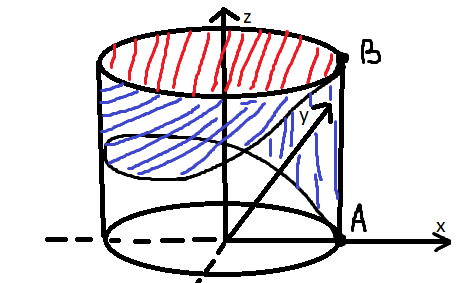
\includegraphics{stokesExample1}\par
Тогда $\int_L \overrightarrow{a} d \overrightarrow{r} = \iint_{\Sigma} rot \overrightarrow{a} \cdot \overrightarrow{n}_0 ds$.\par
Посчитаем ротор, он равен $2 \overrightarrow{k}$.\par
Как видно на картинке выше, нас интересуют две области, на которые и делится $\Sigma$. $\Sigma = \Sigma_1 \cup \Sigma_2$.\par
Рассмотрим по очереди каждую из этих областей:\par
$\Sigma_1 : x^2 + y^2 = a^2, \overrightarrow{n} = (x,y,0), rot \overrightarrow{a} \cdot \overrightarrow{n}_0 = 0$.\par
$\Sigma_2 : z = 2 \pi b, x^2 + y^2 \leq a^2, \overrightarrow{n} = \overrightarrow{k} = \overrightarrow{n}_0, rot \overrightarrow{a} \cdot \overrightarrow{n}_0 = 2$.\par
Тогда $\int_L \overrightarrow{a} d \overrightarrow{r} = \iint_{\Sigma} rot \overrightarrow{a} \overrightarrow{n}_0 ds = \iint_{\Sigma_2} 2 ds = 2 \pi a^2$.\par
2) $\overrightarrow{a} = y \overrightarrow{i} + z \overrightarrow{j} + x \overrightarrow{k}$. Дан куб, ребро имеет длину = 1. Найти циркуляцию вдоль ломаной $C_1CDABB_1A_1D_1$.\par
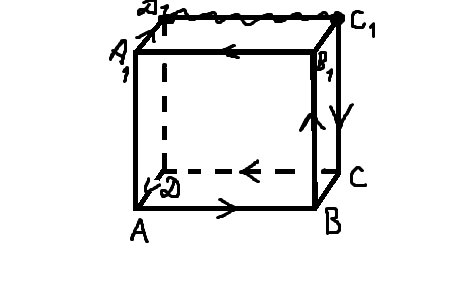
\includegraphics{stokesExample2}\par
Замкнем ломаную, добавив отрезок $D_1C_1$. $L = L_1 \cup D_1C_1$.\par
За поверхность возьмем грани $ABB_1A_1 (\Sigma_1), A_1D_1DA(\Sigma_2)$ и $C_1CDD_1 (\Sigma_3)$.\par
Посчитаем ротор, он равен $-\overrightarrow{i}-\overrightarrow{j}-\overrightarrow{k}$.\par
Тогда $\int_L = \iint_{\Sigma_1} + \iint_{\Sigma_2} + \iint_{\Sigma_3}$.\par
Рассмотрим каждую их областей:\par
$\Sigma_1 : \overrightarrow{n} = -\overrightarrow{i}, rot \overrightarrow{a} \cdot \overrightarrow{n}_0 = 1, \iint_{\Sigma_1} = \iint ds = 1$.\par
$\Sigma_2 : \overrightarrow{n} = \overrightarrow{j}, rot \overrightarrow{a} \cdot \overrightarrow{n}_0 = -1, \iint_{\Sigma_2} = \iint ds = -1$.\par
$\Sigma_3 : \overrightarrow{n} = \overrightarrow{i}, rot \overrightarrow{a} \cdot \overrightarrow{n}_0 = -1, \iint_{\Sigma_3} = \iint ds = -1$.\par
Сложим, получим, что $\int_L = -1$. Осталось посчитать $\int_{D_1C_1} ydx + zdy + xdz = I$.\par
$D_1C_1 : x = 1, z = 1$, тогда $dx = 0, dz = 0$.\par
Отсюда $I = \int_0^1 zdy = 1$. Тогда $\int_{L_1} = \int_L - \int_{D_1C_1} = -2$.\par
\subsection{Примечание к следствию из теоремы Стокса}
\uline{Определение:} область называется линейно-односвязной, если на любой простой замкнутый контур, лежащий в этой области, можно натянуть поверхность, целиком лежащую в этой области.\par
\uline{Утверждение:} следствие выполняется только если область, в которой работаем - линейно-односвязна.
Пример, подтверждающий это:\par
Дана кривая $AB$ и поле $\overrightarrow{a} = (-\frac{y}{x^2 + y^2}, \frac{x}{x^2 + y^2}, z)$. При этом $rot \overrightarrow{a} = 0$.\par
Искомое задание кривой:
$$l :\begin{cases} x^2 + y^2 = a^2 \\ z = a \end{cases}$$
Посчитаем интеграл $\int_{AB} \overrightarrow{a} d \overrightarrow{r}$:
$$\int_{AB} \overrightarrow{a} d \overrightarrow{r} = \int_l -\frac{y}{x^2 + y^2} dx + \frac{x}{x^2 + y^2} dy + zdz = I$$
Параметризуем кривую:
$$\begin{cases} z = a \\ x = a \cos t \\ y = a \sin t \end{cases}$$
Тогда $I = \int_0^{2 \pi} (\frac{a^2 \sin^2 t}{a^2} + \frac{a^2 \cos^2 t}{a^2}) dt + 0$ (так как $dz = 0$, ведь $z$ - константа).
$$I = \int_0^{2 \pi} (\sin^2 t + \cos^2 t) dt = \int_0^{2 \pi} dt = 2 \pi \neq 0$$
Что и требовалось доказать, ведь при $x = 0, y = 0$ у нас поле не определено, тогда область не является линейно-односвязной.\par
\subsection{Линейно b поверхностно односвязные области}
\uline{Определение:} область называется линейно-односвязной, если на любой простой замкнутый контур, лежащий в этой области, можно натянуть поверхность, целиком лежащую в этой области.\par
\uline{Определение:} область $G$ называется поверхностно-односвязной, если для любой простой замкнутой поверхности, ограничивающей некую область $\Omega$, все точки $\Omega$ принадлежат $G$.\par
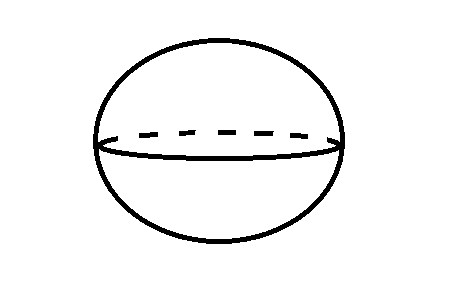
\includegraphics{surfaceSingleConnected1}  шар является примером поверхностно односвязной области.\par
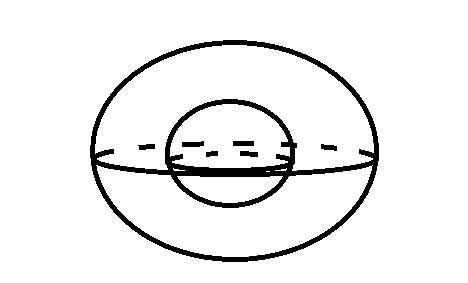
\includegraphics{surfaceNotSingleConnected1} - шар, у которого внутри вырезан шар поменьше является примером поверхностно-неодносвязной области, ведь если взять шар радиусом больше, чем радиус вырезанного шара, но меньше, чем радиус искомого шара, то в нем будут точки из вырезанного шара, которые не принадлежат искомому шару.\par
\section{Потенциальное поле}
Дано векторное поле $\overrightarrow{a} = \overrightarrow{a} (M)$.\par
\uline{Определение:} будем называть $\overrightarrow{a}$ потенциальным, если $\exists U = U(x,y,z)$ такая, что $grad U = \overrightarrow{a}$.\par
\textbf{Важно:} $\overrightarrow{a} = \overrightarrow{\nabla} U$.\par
\uline{Определение:} $U$ - скалярный потенциал векторного поля.\par
\uline{Теорема:} для того, чтобы $\overrightarrow{a}$ было потенциальным, необходимо и (в случае линейной неодносвязности области, в которой задано поле) достаточно, чтобы $rot \overrightarrow{a} = \overrightarrow{0}$.\par
\uwave{Доказательство}:\par
1) Необходимость. Если $\exists U$, то $rot \overrightarrow{a} = rot \ grad \ U = \overrightarrow{\nabla} \times \overrightarrow{\nabla} U = \overrightarrow{0}$.\par
То есть, если поле потенциально (есть скалярный потенциал), то ротор равен нулю.\par
2) Достаточность.\par
$rot \overrightarrow{a} = 0$, область (пусть будет $g$) - линейно-односвязна.\par
Тогда по теореме Стокса $\int_{AB} \overrightarrow{a} d \overrightarrow{r}$ не зависит от пути интегрирования.\par
Теперь просто попробуем найти скалярный потенциал.\par
Возьмем некую функцию $\overset{\sim}{U}(\overset{\sim}{x},\overset{\sim}{y},\overset{\sim}{z})$ и точку $\overset{\sim}{M}=(\overset{\sim}{x},\overset{\sim}{y},\overset{\sim}{z})$.\par
Выберем их такими, что $\overset{\sim}{U} = \int_{M_0}^{\overset{\sim}{M}} \overrightarrow{a} d \overrightarrow{r}$.\par
Теперь докажем, что $\overset{\sim}{U}$ - скалярный потенциал поля $\overrightarrow{a}$:\par
Пусть точка $M_1 = (\overset{\sim}{x}+{\bigtriangleup x}, \overset{\sim}{y}, \overset{\sim}{z})$.\par
Найдем производную $\overset{\sim}{U}$:
$${\bigtriangleup \overset{\sim}{U}} = \overset{\sim}{U} (\overset{\sim}{x}+{\bigtriangleup x}, \overset{\sim}{y}, \overset{\sim}{z})-\overset{\sim}{U}(\overset{\sim}{x},\overset{\sim}{y},\overset{\sim}{z}) = \int_{M_0}^{M_1} - \int_{M_0}^{\overset{\sim}{M}} = I$$
Оба интеграла из разности не зависят от пути интегрирования, тогда:\par
Выберем путь $M_0 \overset{\sim}{M}$ свободно, пусть будет каким угодно.\par
Путь $M_0 M_1 = M_0 \overset{\sim}{M} \cup \overset{\sim}{M} M_1$.\par
$\overset{\sim}{M} M_1$ - отрезок, параллельный оси $x$.\par
Это выглядит так:\par
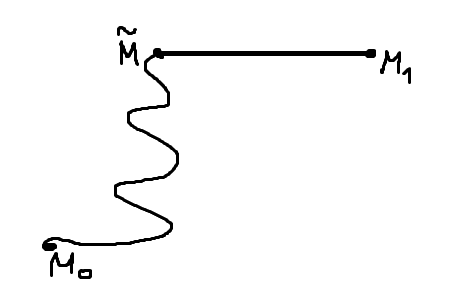
\includegraphics{potentialFields1}\par
Тогда $I = \int_{\overset{\sim}{M}}^{M_1} Pdx + Qdy + Rdz$. Но $dy = 0, dz = 0$, так как меняется только $x$. Тогда $I = \int_{\overset{\sim}{M}}^{M_1} Pdx = \int_{\overset{\sim}{x}}^{\overset{\sim}{x}+{\bigtriangleup x}} P(x, \overset{\sim}{y}, \overset{\sim}{z}) = P(\overset{\sim}{x}+\theta \bigtriangleup x, \overset{\sim}{y}, \overset{\sim}{z}) \bigtriangleup x$ (по теореме о среднем), где $0 < \theta < 1$.\par
Тогда $\frac{\partial \overset{\sim}{U}}{\partial x} = \lim_{\bigtriangleup x \to 0} \frac{\bigtriangleup \overset{\sim}{U}}{\bigtriangleup x} = \lim_{\bigtriangleup x \to 0} P(\overset{\sim}{x}+\theta \bigtriangleup x, \overset{\sim}{y}, \overset{\sim}{z}) = P(\overset{\sim}{x}, \overset{\sim}{y}, \overset{\sim}{z})$.\par
Аналогично получится и для $y$ и $z$. Тогда $grad \overset{\sim}{U} = \overrightarrow{a}$, значит, $\overset{\sim}{U}$ - скалярный потенциал, то есть мы нашли искомую функцию, что и требовалось доказать.\par
\textbf{Важно:} если $U$ - скалярный потенциал, то $U + c$, где $c = const$ - тоже скалярный потенциал.\par
\uline{\textbf{ПРИМЕР:}}\par
$\overrightarrow{a} = (y+z) \overrightarrow{i} + (x+z) \overrightarrow{j} + (x+y)\overrightarrow{k}$. Задача: убедиться, что данное поле является потенциальным и найти его потенциал.\par
Решение:\par
1) $rot \overrightarrow{a} = \overrightarrow{0}$ (здесь нужно вычислить определитель матрицы), следовательно, поле потенциальное.\par
2) $U = \int_{(0,0,0)}^{(x_0,y_0,z_0)} (y+z) dx + (x+z) dy + (x + y) dz = \int_{l_1} + \int_{l_2} + \int_{l_3}$. Выберем путь, по которому будем двигаться из точки $(0,0,0)$ в точку $(x_0,y_0,z_0)$: самый хороший путь - это двигаться вдоль координатных осей:\par
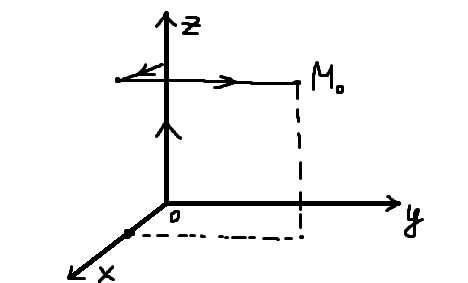
\includegraphics{scalarPotential1}\par
Тогда посчитаем каждый из трех интегралов:\par
a) $x = 0, y = 0, \Rightarrow dx = 0, dy = 0. \ 0 \leq z \leq z_0$. Тогда $\int_{l_1} = 0dz = 0$.\par
b) $z = z_0, y = 0, \Rightarrow dz = 0, dy = 0. \ 0 \leq x \leq x_0$. Тогда $\int_{l_2} = \int_0^{x_0} z_0 x = z_0 x_0$.\par
c) $x = x_0, z = z_0, \Rightarrow dz = 0, dx = 0. \ 0 \leq y \leq y_0$. Тогда $\int_{l_3} = \int_0^{y_0} (x_0 + z_0) = x_0 y_0 + z_0 y_0$.\par
Сложим три интеграла, получим, что $U = xy + xz + yz$, что и будет ответом.\par
\section{Соленоидальное поле}
Дано $\overrightarrow{a}$ - векторное поле, заданное на $g$ - поверхностно-односвязной области.\par
\uline{Определение:} векторное поле будем называть соленоидальным, если его поток через любую простую, кусочно-гладкую, замкнутую поверхность равен нулю:
$$\iint_S \overrightarrow{a} \overrightarrow{n_0} ds = 0$$
\uline{Теорема 1:} для того, чтобы поле было соленоидальным, необходимо и достаточно, чтобы выполнялось условие:
$$div \overrightarrow{a} = 0$$
\uwave{Доказательство}:\par
1) $$\iint_S \overrightarrow{a} \overrightarrow{n_0} ds = \iiint_V div \overrightarrow{a} d V = 0, \Rightarrow div \overrightarrow{a} = 0$$
2) $$div \overrightarrow{a} = 0, \Rightarrow \iint_S \overrightarrow{a} \overrightarrow{n_0} ds = 0, \Rightarrow \overrightarrow{a} - \text{соленоидальное}$$
\uline{Определение:} $\overrightarrow{H}$ будем называть векторным потенциалом поля $\overrightarrow{a}$, если $rot \overrightarrow{H} = \overrightarrow{a}$.\par
\textbf{Важно:} если $\overrightarrow{H}$ - векторный потенциал, то $\overrightarrow{H_1} = \overrightarrow{H} + gradU$ (где $U$ - какая-то скалярная функция) - тоже векторный потенциал.\par
\uwave{Доказательство}:
$$rot \overrightarrow{H_1} = rot (\overrightarrow{H} + gradU) = rot \overrightarrow{H} + rot \ gradU (=0) = rot \overrightarrow{H} = \overrightarrow{a}$$
\uline{Теорема 2:} для того, чтобы поле было соленоидальным, необходимо и достаточно, чтобы существовал векторный потенциал.\par
\uwave{Доказательство}:\par
1) $$div \overrightarrow{a} = div \ rot \overrightarrow{H} = \overrightarrow{\nabla} \cdot \overrightarrow{\nabla} \times \overrightarrow{H} = 0$$
А по теореме 1, если дивергенция равна нулю, то поле соленоидальное.\par
2) $\overrightarrow{a}$ - соленоидальное.\par
Будем искать $\overrightarrow{H}$ в виде $\overrightarrow{H} = (H_x, H_y, 0)$.
$$rot \overrightarrow{H} = -\overrightarrow{i} \frac{\partial H_y}{\partial x} + \overrightarrow{j} \frac{\partial H_x}{\partial z} + \overrightarrow{k} (\frac{\partial H_y}{\partial x} - \frac{\partial H_x}{\partial y}) = P\overrightarrow{i} + Q\overrightarrow{j}+R\overrightarrow{k}$$
Отсюда \par$\frac{\partial H_y}{\partial z} = -P, \Rightarrow H_y = -\int Pdz + \varphi(x,y) \ (\varphi(x,y)$ - произвольная функция).\par
\indent $\frac{\partial H_x}{\partial z} = Q, \Rightarrow H_x = \int Qdz + \psi(x,y) \ (\psi(x,y)$ - произвольная функция).
$$\frac{\partial H_y}{\partial x} - \frac{\partial H_x}{\partial y} = R, \Rightarrow -\int P_x dz + \varphi_x(x,y) - \int Q_y dz + \psi_y(x,y)$$
Таким образом, мы нашли $\overrightarrow{H}$.\par
\uline{\textbf{ПРИМЕР:}}\par
$\overrightarrow{a} = 2 z \overrightarrow{i} + 3 y^2 \overrightarrow{k} = (2z, 0, 3y^2)$.\par
Найти векторный потенциал. Решение:\par
$H_x = \int 0 + \psi (x,y)$.\par
$H_y = -\int 2z dz + \varphi (x,y) = -z^2 + \varphi(x,y)$.\par
$H_z = 0$.
$$-0 + \varphi_x - 0 - \psi_y = 3y^2$$
$$\varphi_x - \psi_y = 3y^2$$
Обе функции произвольные, поэтому, пусть $\varphi \equiv 0, \psi = -y^3$.\par
Тогда, ответ: $\overrightarrow{H} = (-y^3, -z^2, 0)$.\par
\section{Интегралы с параметрами}
Дальше (похоже, до конца семестра) мы будем заниматься интегралами с параметрами.\par
\section{Равномерная сходимость семейства функций}
\subsection{Определение равномерной сходимости}
Дана функция $f(x,y)$ - на первый взгляд, функция двух переменных, однако, $x \in X$ - аргумент, а $y \in Y$ - число, параметр.\par
Например, если $Y = N$ (натуральные числа), то $f (x,n) = f_n (x)$ - функциональная последовательность.\par
Возьмем некую точку $y_0$ - точку сгущения $Y$ (по сути, точка сгущения $\sim$ предельная точка множества).\par
Тогда функцию $\varphi (x)$, такую, что:
$$\forall x \in X \ f(x,y)_{y\to y_0} \to \varphi(x)$$
будем называть \textbf{поточечным} пределом функции $f$.\par
\uline{Определение:}
$f(x,y)$ сходится равномерно на $X$ при $y \to y_0$, если:\par
1) $f(x,y)_{y\to y_0} \to \varphi (x) \forall x$ (сходится поточечно).\par
2) $$\forall \varepsilon > 0 \ \exists \delta > 0 : 0 < |y-y_0| < \delta \Rightarrow |f(x,y) - \varphi(x)|<\varepsilon \ \  \forall x$$
\uline{\textbf{ПРИМЕР:}}\par
$f(x,y) = \frac{3x+y}{x+y}; Y = (0;1), y_0 = 0$. Выяснить, сходится ли равномерно функция на множестве $X$, если $X$:\par
1) $X = (1,2)$.\par
Найдем поточечный предел $f$:
$$\lim_{y\to y_0} f = \frac{3x}{x} = 3 = \varphi(x)$$
Подставим поточечный предел в определение:
$$|f(x,y)-\varphi(x)| = |\frac{3x+y}{x+y} - 3| = \frac{2y}{x+y} < \varepsilon \ \ \forall x \in (1,2)$$
$$\frac{2y}{x+y} < \frac{2y}{1+y} < \frac{2y}{1} < \varepsilon$$
Тогда возьмем $\delta = \frac{\varepsilon}{2}$, значит, мы нашли $\delta$, удовлетворяющую условию, значит, $f$ равномерно сходится на $X$.\par
2) $X = (0,1)$.\par
Докажем, что нет равномерной сходимости на этом множестве. Для этого докажем отрицание определения равномерной сходимости:
$$\exists \varepsilon_0 > 0 \ \forall \delta > 0; \exists y_{\delta} \in U_{\delta} (y_0); \exists x_{\delta} \Rightarrow |f(x_{\delta}, y_{\delta})-\varphi(x_{\delta})| \geq \varepsilon_0$$
Пусть $\delta_n = \frac{1}{n}, y_n = \frac{1}{n+1}, x_n = \frac{1}{n+1}$. Тогда $\frac{2y}{x+y} = 1 = \varepsilon_0$. То есть мы нашли $\varepsilon_0$, а значит, доказали отрицание, а значит, $f$ не сходится равномерно на данном $X$.\par
\subsection{Признаки равномерной сходимости}
1) Запишем очевидное неравенство:\par
Пусть $|f(x,y)-\varphi(x)|<\varepsilon \ \ \forall x \in X$. Тогда
$$|f(x,y)-\varphi(x)| \leq sup_{x \in X} |f(x,y) - \varphi(x)| = g(y)$$
\uline{Утверждение}: семейство функций сходится равномерно к $\varphi(x)$ на множестве $X$ тогда и только тогда, когда:
$$\forall \varepsilon > 0 \ \exists \delta > 0 \ y \in \overset{o}{U_{\delta}}(y_0) \Rightarrow |g(y)|<\varepsilon$$
Например, $sup_{x\in (1;2)} \frac{2y}{x+y} = \frac{2y}{1+y} < \varepsilon$. Но\par
$sup_{x \in (0;1)} \frac{2y}{x+y} = 2$ - не стремится к нулю.\par
2) \uline{Теорема (признак Коши)}:\par
Для того, чтобы семейство функций равномерно сходилось на $X$ при $y \to y_0$, необходимо и достаточно, чтобы выполнялось условие:
$$\forall \varepsilon > 0 \ \exists \delta > 0 : \forall y^{'}, y^{''} \in U_{\delta}(y_0) \Rightarrow |f(x,y^{'})-f(x,y^{''})| < \varepsilon \ \ \forall x \in X$$
\uwave{Доказательство}:\par
$\Romannum{1}. \Rightarrow$\par
Если семейство функций сходится равномерно, то
$$\forall \varepsilon > 0 \ \exists \delta > 0 \  \forall y \in \overset{o}{U_\delta}(y_0): |f(x,y)-\varphi(x)|<\frac{\varepsilon}{2}$$
Возьмем две точки из $\overset{o}{U_\delta}(y_0)$ - $y^{'}$ и $y^{''}$.\par
Тогда $|f(x,y^{'})-\varphi(x)| < \frac{\varepsilon}{2}$,\par
$\indent |f(x,y^{''})-\varphi(x)| < \frac{\varepsilon}{2}$,
$$|f(x,y^{'})-f(x,y^{''})| \leq |f(x,y^{'})-\varphi(x)| + |f(x,y^{''})-\varphi(x)| < \frac{\varepsilon}{2} + \frac{\varepsilon}{2} < \varepsilon$$
Доказано.\par
$\Romannum{2}. \Leftarrow$\par
Теперь дано условие Коши.\par
Возьмем $x \in X$ и зафиксируем его. Тогда для фиксированного $x$ выполняется:
$$|f(x,y^{'})-f(x,y^{''})| < \varepsilon \Rightarrow |g(y^{'})-g(y^{''})| < \varepsilon$$
Отсюда следует, что у функции $g$ есть предел при $y \to y_0$.\par
Получается, что для каждого такого фиксированного $x \in X \\ \exists \lim_{y \to y_0} f(x,y) = \varphi(x)$.\par
Осталось доказать вторую часть определения равномерной сходимости:\par
Для этого в выражении $|f(x,y^{'})-f(x,y^{''})| < \frac{\varepsilon}{2}$ перейдем к пределу:\par
Пусть $y \to y_0$, тогда $|f(x,y^{'})-\varphi(x)| \leq \frac{\varepsilon}{2} < \varepsilon$, что и требовалось доказать.\par
Теорема доказана.\par
3) Обозначим за $\mapsto$ равномерную сходимость.\par
\uline{Утверждение}: для того, чтобы $f(x,y)$ сходилась равномерно к $\varphi(x)$ на множестве $X$ и при $y \to y_0$, необходимо и достаточно, чтобы выполнялось условие:
$$\forall y_n \to y_0 \ f(x,y_n) = f_n(x)_{n \to \infty} \mapsto \varphi(x) \ \forall x \in X$$
Здесь $y_n$ - последовательность из $Y$.\par
\uwave{Доказательство}:\par
$\Romannum{1}. \Rightarrow$\par
Если $f$ равномерно сходится, то это значит, что:
$$\forall \varepsilon > 0 \ \exists \delta > 0 \ \forall y \in \overset{o}{U_\delta}(y_0) \ |f(x,y)-\varphi(x)| < \varepsilon$$
Возьмем последовательность $y_n \to y_0$ и по $\delta$, которую мы нашли, найдем $n_0$, такой, что:
$$\forall n \geq n_0 \ y_n \in \overset{o}{U_\delta}(y_0)$$
А это означает, что $\forall x \ |f(x,y_n)-\varphi(x)| < \varepsilon$, что и требовалось доказать.\par
$\Romannum{2}. \Leftarrow$\par
Теперь дано: $\forall y_n \to y_0 \ f(x,y_n) = f_n(x)_{n \to \infty} \mapsto \varphi(x)$.\par
Докажем от противного, что $f(x,y) \mapsto \varphi(x)$.\par
Пусть $f$ сходится, но не равномерно, тогда снова попытаемся доказать отрицание:
$$\exists \varepsilon_0 > 0 \ \forall \delta > 0; \exists y_{\delta} \in U_{\delta} (y_0); \exists x_{\delta} \Rightarrow |f(x_{\delta}, y_{\delta})-\varphi(x_{\delta})| \geq \varepsilon_0$$
Поскольку мы наложили условия на $x_\delta$ и $y_\delta$, то можем взять какие-то последовательности $x_n, y_n$, а $\delta_n$ взять равное $\frac{1}{n}$.\par
Тогда:
$$|f(x_{n}, y_{n})-\varphi(x_{n})| \geq \varepsilon_0$$
Но это противоречит условию, ведь по условию $f_n$ равномерно сходится к $\varphi$. Теорема доказана.\par
\uline{Следствие}:\par
Пусть $f(x,y)$ непрерывна по $x$ на множестве $X$, а так же эти $f(x,y) \mapsto \varphi(x)$ при $y \to y_0$ на $X$.\par
Тогда $\varphi(x)$ непрерывна на $X$.\par
4) \uline{Утверждение}: если рассматривать $f(x,y)$ на прямоугольнике $[a;b] \times [c;d]$ как функцию двух переменных и предположить, что она на нем непрерывна, то
$$f(x,y)_{y \to y_0} \mapsto \varphi_{y_0}(x)$$
Здесь $y_0 \in [c;d]$.\par
\uwave{Доказательство}:\par
Данный прямоугольник - компактное множество. А если функция непрерывна на компакте равномерно непрерывна:
$$\forall \varepsilon > 0 \ \exists \delta > 0 \ \forall x^{'}, x^{''}:|x^{'} - x^{''}| < \delta; \forall y^{'}, y^{''}:|y^{'} - y^{''}| < \delta \Rightarrow$$
$$\Rightarrow |f(x^{'}, y^{'})-f(x^{''},y^{''})|<\varepsilon$$
Возьмем $x^{'} = x^{''} = x, y^{''} = y_0, y^{'} = y$.\par
Тогда $|f(x,y)-f(x,y_0)|<\varepsilon$, но $f(x,y_0) = \varphi_{y_0}(x)$, тогда:
$$|f(x,y)-\varphi_{y_0}(x)| < \varepsilon \ \forall x \in [a;b]$$
Но это и означает равномерную сходимость (по определению), что и требовалось доказать.\par
\section{Интеграл с переменным верхним пределом}
Дана $f(x,y)$ - интегрируемая по $x \in [a;b] \ \forall y \in Y$.\par
Тогда рассмотрим интеграл:\par
$I(y) = \int_a^b f(x,y) dx$ - собственный интеграл с параметром $y$.\par
\uwave{Свойства}:\par
1) \uline{Теорема 1}: если $f(x,y) \mapsto \varphi(x)$ при $y \to y_0$, то
$$\lim_{y \to y_0} I(y) = \int_a^b \varphi (x) dx$$
Эта теорема дает нам возможность менять местами знаки предела и интеграла в случае, когда $f$ равномерно сходится:
$$\lim_{y \to y_0} \int_a^b f(x,y) dx = \int_a^b \lim_{y \to y_0} f(x,y) dx$$
\uwave{Доказательство}:\par
Оценим $|I(y)-\int_a^b \varphi(x)dx|$:
$$|I(y)-\int_a^b \varphi(x)dx| \ |\int_a^b f(x,y)dx-\int_a^b \varphi(x)dx| =$$
$$= |\int_a^b (f(x,y)-\varphi(x))dx| \leq \int_a^b |(f(x,y)-\varphi(x))|dx$$
Но $f(x,y) \mapsto \varphi(x) \Rightarrow |f(x,y) - \varphi(x)| < \varepsilon$.\par
Пусть $\varepsilon = \frac{\varepsilon}{b-a}$:
$$\int_a^b |(f(x,y)-\varphi(x))|dx < \int_a^b \frac{\varepsilon}{b-a} dx = \varepsilon$$
Значит, $\lim_{y \to y_0} I(y) = \int_a^b \varphi (x) dx$, что и требовалось доказать.\par
\uwave{Следствия}:\par
a) Если $f$ непрерывна на прямоугольнике $[a;b] \times [c;d]$, то можно переставить знаки интегрирования и предела местами.\par
b) Если в точке $y_0 \  f(x,y)$ непрерывна, то из того, что $f(x,y) \mapsto \varphi(x)$ следует, что:
$$\lim_{y \to y_0} I(y) = \int_a^b f(x,y_0) dx = I(y_0)$$
Отсюда следует, что $I$ непрерывен в точке $y_0$ (по определению непрерывности в точке).\par
2) \uline{Теорема 2}: если $f(x,y)$ непрерывна относительно $x$ и $y$ на прямоугольнике $[a;b] \times [c;d]$, то $I(y) = \int_a^b f(x,y) dx$ можно интегрировать по $y$:
$$\exists \int_c^d dy \int_a^b f(x,y) dx = \int_a^b dx \int_c^d f(x,y) dy$$
Это повторные интегралы для двойного интеграла $\iint_{[a;b]\times [c;d]} f(x,y) dxdy$.\par
Другими словами,\par $$\iint_{[a;b]\times [c;d]} f(x,y) dxdy = \int_c^d dy \int_a^b f(x,y) = \int_a^b dx \int_c^d f(x,y) dydx$$
3) \uline{Теорема 3}:\par
Пусть $f(x,y)$ непрерывна по $x$ на $[a;b]$ для любых $y$ из $[c;d]$, а $f^{'}_y(x,y)$ непрерывна по $x$ и $y$ на прямоугольнике $[a;b] \times [c;d]$.\par
Тогда существует $I^{'}_y (y) \ \forall y\in [c;d]$:
$$I^{'}_y (y) = \int_a^b f^{'}_y (x,y) dx$$
То есть, другими словами, можно поменять дифференцирование и интегрирование местами:\par
$(\int f)^{'} = \int f^{'}$ - это называется правило Лейбница.\par
\uwave{Доказательство}:
$$I^{'}_y(y_0) = \lim_{{\bigtriangleup y} \to 0} \frac{{\bigtriangleup I(y_0)}}{{\bigtriangleup y}} = \lim_{{\bigtriangleup y} \to 0} \frac{I(y_0+{\bigtriangleup y}) - I(y_0)}{{\bigtriangleup y}} = ?$$
Распишем $\frac{{\bigtriangleup I(y_0)}}{{\bigtriangleup y}}$:
$$\frac{{\bigtriangleup I(y_0)}}{{\bigtriangleup y}} = \frac{\int_a^b f(x, y_0 + {\bigtriangleup y}) dx - \int_a^b f(x,y_0) dx}{{\bigtriangleup y}} =$$
$$= \int_a^b \frac{f(x,y_0+{\bigtriangleup y}) - f(x,y_0)}{{\bigtriangleup y}} dx = \int_a^b \frac{f^{'}_y (x, y_0 + \theta {\bigtriangleup y}) {\bigtriangleup y} dx}{{\bigtriangleup y}} =$$
$$= \int_a^b f^{'}_y (x, y_0 + \theta {\bigtriangleup y}) dx, \ 0 < \theta < 1 (\text{по теореме о среднем})$$
Тогда $I^{'}_y (y_0) = \lim_{{\bigtriangleup y} \to 0} \int_a^b f^{'}_y (x, y_0 + \theta {\bigtriangleup y}) dx = \int_a^b \lim_{{\bigtriangleup y} \to 0}  f^{'}_y (x, y_0 + \theta {\bigtriangleup y}) dx =\\= \int_a^b f^{'}_y (x,y_0) dx$, что и требовалось доказать.\par
\uwave{Замечание}:\par
Если пределы интегрирования зависят от $y$, вот таким образом:
$$I(y) = \int_{u(y)}^{v(y)} f(x,y) dx = F(y,u,v)$$
Тогда $\frac{dF}{dy} = \frac{\partial F}{\partial y} + \frac{\partial F}{\partial u} \frac{du}{dy} + \frac{\partial F}{\partial v} \frac{dv}{dy} = \int_u^v f^{'}(x,y) dx + f(v,y) v^{'}_y - f(u,y) u^{'}_y$.\par
Это следует из теоремы Барроу (по словам некоторых, самой великой теоремы матанализа, а значит надо учить):\par
\uline{\textbf{Теорема Барроу}}:
$$(\int_a^x f(t) dt)^{'}_x = f(x)$$
$$(\int_x^b f(t) dt)^{'}_x = f(-x)$$
\uline{\textbf{ПРИМЕРЫ (здесь их много, 5 штук)}}:\par
1) $I(y) = \int_0^1 \ln(x^2+y^2) dx; \ y\in (0;1]$.\par
Посчитаем этот интеграл:
$$\int_0^1 \ln (x^2+y^2) dx = x \ln (x^2 + y^2) |_0^1 - 2 \int \frac{xdx}{x^2+y^2} = \ln (1+y^2) - 2 + y \arctg \frac{1}{y}$$
Хотим узнать, как эта функция ведет себя в нуле, устремим $y$ к нулю, тогда $I(y) \to 0$, то есть, $0$ - точка устранимого разрыва.\par
Тогда $I(y) = \begin{cases} \ln (1+y^2) - 2 + y \arctg \frac{1}{y}, y \neq 0 \\ -2, y = 0 \end{cases}$.\par
Значит, $I(y)$ непрерывна на $[0;1]$.\par
Теперь проверим дифференцируемость:\par
$y \neq 0, y \in [\delta; 1]$. Тогда на прямоугольнике $[0;1] \times [\delta; 1]$ функция $\ln (x^2+y^2)$ непрерывна по $y$, а функция $\frac{2y}{x^2+y^2}$ непрерывна по $x$ и по $y$.\par
Тогда $I^{'}_y(y) = \int_0^1 \frac{2y}{x^2+y^2}$, рассмотрим её поведение в нуле:\par
$y_0 = 0$.
$$I^{'}_y(y) = \frac{2y}{x^2+y^2} + \arctg \frac{1}{y} - \frac{y}{1+y^2} = \frac{y}{1+y^2} + \arctg \frac{1}{y}$$
Очевидно, эта функция не непрерывна в нуле, устремим $y$ к нулю, тогда $I^{'}_y(0) \to \frac{\pi}{2}$.\par
С другой стороны, $I^{'}_y(0) = \int_0^1 \frac{2y}{x^2+y^2} dx = 0$.\par
Получили разные ответы. Это потому, что на самом деле мы не могли здесь пользоваться теоремой, ведь нарушается условие непрерывности $f^{'}_y$ по $x$ и по $y$.\par
2) $\int_0^1 \frac{x^b-x^a}{\ln x} dx, \ b > a > 0$.
$$\frac{x^b - x^a}{\ln x} = \int_a^b x^y dy$$
Тогда $\int_0^1 \frac{x^b-x^a}{\ln x} = \int_0^1 dx \int_a^b x^y dy = \int_0^1 dy \int_a^b x^y dx = \int_a^b \frac{x^{y+1}}{y+1} |_0^1 dy = \int_a^b \frac{1}{y+1} dy = \ln \frac{b+1}{a+1}$.\par
С другой стороны,
$$I(a,b) = \int_0^1 \frac{x^b - x^a}{\ln x} dx \Rightarrow I^{'}_b (a,b) = \int_0^1 x^b dx = \frac{x^{b+1}}{b+1} |_0^1 = \frac{1}{b+1}$$
Тогда $\int I^{'}_b (a,b) = \int \frac{db}{b+1} = \ln (b+1) + C$. Найдем $C$:
$$I(a,a) = \ln (a+1) + C = 0 \Rightarrow C = -\ln(a+1)$$
Отсюда $I(a,b) = \ln (b+1) - \ln(a+1) = \ln \frac{b+1}{a+1}$, получили то же самое.\par
3) $\int_0^1 \frac{\arctg x}{x \sqrt{1-x^2}} dx$.\par
Рассмотрим $\frac{\arctg x}{x}$:
$$\frac{\arctg x}{x} = \int_0^1 \frac{dy}{1+x^2y^2}, \text{тогда} \int_0^1 \frac{\arctg x}{x \sqrt{1-x^2}} dx = \int_0^1 dx \int_0^1 \frac{dy}{(1+x^2y^2)\sqrt{1-x^2}} = $$
$$= \int_0^1 dx \int_0^1 f(x,y) g(x) dy = \int_0^1 dy \int_0^1 f(x,y) g(x) dx = \int_0^1 dy \int_0^1 \frac{dx}{(1+x^2y^2)\sqrt{1-x^2}}=$$
$$= -\int_0^1 dy \int_0^{- \infty} \frac{dt}{t^2(y^2+1)+1} (\text{подстановка Абеля}) = \int_0^1 dy \int_0^\infty \frac{dt}{t^2(y^2+1)+1} = $$
$$= \int_0^1 \frac{\arctg (t \sqrt{y^2+1})}{\sqrt{y^2+1}} |_0^{\infty} dy = \int_0^1 \frac{\pi}{2\sqrt{y^2+1}} dy = \frac{\pi}{2} \int_0^1 \frac{dy}{\sqrt{y^2+1}} = \frac{\pi}{2} \ln(1+\sqrt{2})$$
Второй способ:\par
Найдем $I^{'}_y$:
$$I^{'}_y = \int_0^1 \frac{1}{1+x^2y^2} \frac{1}{\sqrt{1-x^2}} dx = \frac{\pi}{2} \frac{1}{\sqrt{y^2+1}}$$
Получили производную, осталось найти саму функцию:
$$I(y) = \int I^{'}_y = \frac{\pi}{2} \ln (y + \sqrt{y^2+1}) + C$$
Найдем $C$:\par
$I(0) = 0, \Rightarrow C = 0$, а наша цель - $I(1)$.
$$I(1) = \frac{\pi}{2} \ln(1+\sqrt{2})$$
4) $I(a) = \int_0^{\frac{\pi}{2}} \ln (a^2 - \sin^2 t)dt, a>0$.
$$I^{'}_y(a) = \int_0^{\frac{\pi}{2}} \frac{2a}{a^2-\sin^2t}dt = 2a \int_0^{\frac{\pi}{2}} \frac{dt}{a^2-\sin^2t} = \frac{\pi}{\sqrt{a^2-1}}$$
$$I(a) = \int I^{'}_y = \pi \ln (a+\sqrt{a^2-1}) + C$$
С другой стороны, $I(a) = \int_0^{\frac{\pi}{2}} \ln (a^2 - \sin^2 t)dt = \int_0^{\frac{\pi}{2}} \ln (a^2 (1 - \frac{1}{a^2} \sin^2 t)) dt = \pi \ln a + \int_0^{\frac{\pi}{2}} \ln (1 - \frac{1}{a^2} \sin^2 t) dt$\par
Устремим $a$ к $+\infty$, тогда $\ln (1 - \frac{1}{a^2} \sin^2 t) \to 0$. Выясним, равномерно ли сходится семейство функций:
$$|\ln (1 - \frac{1}{a^2} \sin^2t)| \leq |\ln (1 - \frac{1}{a^2})| < \varepsilon$$
Следовательно, сходимость равномерная.\par
Тогда $C = I(a) - \pi \ln (a+\sqrt{a^2-1}) = \pi \ln a - \pi \ln (a + \sqrt{a^2-1}) + \int_0^{\frac{\pi}{2}} \ln (1 - \frac{1}{a^2} \sin^2 t) dt = \pi \ln \frac{a}{a+\sqrt{a^2-1}} + \int_0^{\frac{\pi}{2}} \ln (1 - \frac{1}{a^2} \sin^2 t) dt$.\par
При $a \to \infty$ первое слагаемое стремится к $\ln \frac{1}{2}$, а второе к нулю, тогда $C = \ln \frac{1}{2}$, а $I(a) = \pi \ln \frac{a+\sqrt{a^2-1}}{2}$.\par
\section{Несобственный интеграл}
\subsection{Определение несобственного интеграла}
Возьмем интеграл $\int_a^b f(x) dx$, у которого либо $b = +\infty$, либо $f(x) \to \infty$ при $x\to b-0$.\par
При этом $f(x)$ интегрируема на $[a;c]$, где $a<c<b$.\par
\uline{Определение}:\par
Предел $\lim_{c \to b-0} \int_a^c f(x) dx$ будем называть несобственным интегралом. Если этот предел существует, то будем говорить, что интеграл сходится, иначе расходится.\par
Теперь рассмотрим функцию двух переменных $f(x,y), x \in [a;b],\\ -\infty < b \leq +\infty$.\par
Тогда существует $I(y) = \int_a^b f(x,y) dx = \lim_{c \to b-0} \int_a^c f(x,y) dx$.\par
\uline{\textbf{ПРИМЕР}}:
$$I(y) = \int_0^{\infty} y e^{-xy} dx = \int_0^{\infty} e^{-xy} d(xy) = e^{-xy} |_0^{\infty} = 1$$
То есть, $\int_0^{\infty} = \begin{cases} 0, y = 0 \\ 1, y \neq 0 \end{cases}$.\par
\uline{Определение}: будем говорить, что несобственный интеграл сходится равномерно на $Y$, если:\par
1) Он сходится.\par
2) $\forall \varepsilon > 0 \ \exists \delta > 0, b-\delta > a, \forall c  \ 0 < b - \delta < c < b : | \int_c^b f(x,y) dx| < \varepsilon \ \forall y \in Y$.\par
\uline{\textbf{ПРИМЕРЫ}}:\par
1) $\int_1^\infty \frac{y^2-x^2}{(x^2+y^2)^2} dx$.\par
Оценим этот интеграл:
$$|\int_1^\infty \frac{y^2-x^2}{(x^2+y^2)^2} dx| \leq \int_1^\infty \frac{|y^2-x^2|}{(x^2+y^2)^2} dx \leq \int_1^\infty \frac{dx}{(x^2+y^2)^2} \leq \int_1^\infty \frac{dx}{x^2} < \varepsilon$$
Тогда этот интеграл равномерно сходится.\par
2) $\int_0^{\infty} y e^{-xy} dx$.\par
Докажем, что этот интеграл не сходится равномерно, для этого докажем отрицание определения:
$$\exists \varepsilon_0 \ \forall \delta \ \exists C_\delta; \exists y_\delta : |\int_{c_\delta}^\infty y_\delta e^{-xy_\delta} dx | \geq \varepsilon_0$$
Пусть $xy_\delta = t$:
$$I = \int_{c_\delta y_\delta}^\infty e^{-t} dt = e^{-c_\delta y_\delta}$$
Отсюда очевидно, что можно найти $C_\delta$ и $y_\delta$ такие, что $e^{-c_\delta y_\delta} \geq \varepsilon_0$, тогда интеграл не сходится равномерно.\par
\subsection{Признаки равномерной сходимости несобственных интегралов}
1) Признак Коши.\par
\uline{Утверждение}: для того, чтобы несобственный интеграл $\int_a^b f(x,y) dx$ равномерно сходился на $Y$, необходимо и достаточно, чтобы:
$$\forall \varepsilon > 0 \ \exists \delta > 0 \ \forall c_1, c_2 \ a < b-\delta < c_1,c_2<b : |\int_{c_1}^{c_2} f(x,y) dx | < \varepsilon \ \forall y \in Y$$
\uwave{Доказательство}:\par
$\Romannum{1}. \Rightarrow$\par
Пусть $\int_a^b f(x,y)dx$ сходится равномерно на $Y$. Тогда по определению:
$$\forall \varepsilon > 0 \ \exists \delta \ \forall c \ a < b -\delta < c < b : |\int_a^b f(x,y) dx| < \frac{\varepsilon}{2}$$
Возьмем два разных $c$: $c_1$ и $c_2$ такие, что $a < b-\delta < c_1,c_2 < b$, тогда:
$$|\int_{c_1}^{c_2} \leq |\int_{c_1}^b| + |\int_b^{c_2}| < \frac{\varepsilon}{2} + \frac{\varepsilon}{2} = \varepsilon$$
Что и требовалось доказать.\par
$\Romannum{2}. \Leftarrow$\par
Теперь нам дано, что $|\int_{c_1}^{c_2} f(x,y) dx| < \frac{\varepsilon}{2}$.\par
Пусть $c_2 \to b-0$, тогда
$$|\int_{c_1}^\infty f(x,y) dx | \leq \frac{\varepsilon}{2} < \varepsilon \ \forall y \in Y$$
Что и требовалось доказать.\par
2) Признак Вейерштрасса:\par
\uline{Утверждение}: если существует функция $\varphi(x)$, которая не имеет особых точек кроме $b$, а так же $\int_a^b \varphi(x)$ сходится, то и интеграл $\int_a^b f(x,y) dx$ сходится равномерно.\par
\uwave{Доказательство}:\par
Используем признак Коши, оценим интеграл:
$$|\int_{c_1}^{c_2} f(x,y) dx| \leq \int_{c_1}^{c_2} |f(x,y)| dx \leq \int_{c_1}^{c_2} \varphi(x) dx < \varepsilon$$
Тогда по признаку Коши этот интеграл сходится равномерно.\par
В следующих двух признаках дан интеграл $I = \int_a^b f(x,y) g(x,y) dx$, а так же некоторые условия.\par
В доказательстве обоих понадобится следующая выкладка:\par
Распишем $\int_{c_1}^{c_2} f(x,y) g(x,y) dx$:
$$\int_{c_1}^{c_2} f(x,y) g(x,y) dx = g(c_1,y) \int_{c_1}^{\xi} f(x,y) dx + g(c_2,y) \int_{\xi}^{c_2} f(x,y)dx$$
$$|\int_{c_1}^{c_2} f(x,y) g(x,y) dx|\leq |g(c_1,y)| \cdot |\int_{c_1}^{\xi} f(x,y) dx| + |g(c_2,y) | \cdot |\int_{\xi}^{c_2} f(x,y)dx|$$
3) Признак Абеля.\par
a) $g(x,y)$ монотонна по $x$.\par
$\indent |g(x,y)|<C$\par
б) $\int_a^b f(x,y) dx$ сходится равномерно на $Y$.\par
\uline{Утверждение}: $I$ сходится равномерно.\par
\uwave{Доказательство}:\par
$f(x,y)dx$ сходится равномерно, а $|g(c_1,y)| < C; \ |g(c_2,y)| < C$.\par
Тогда по признаку Коши:
$$|\int_{c_1}^{\xi} f(x,y)dx| < \frac{\varepsilon}{2C}; \ |\int_{c_2}^{\xi} f(x,y)dx| < \frac{\varepsilon}{2C}$$
Отсюда $|\int_{c_1}^{c_2} f(x,y)g(x,y) dx| < \frac {C \varepsilon}{2C} + \frac {C \varepsilon}{2C} = \varepsilon$, что и требовалось доказать.\par
4) Признак Дирихле.\par
а) $g(x,y)$ монотонна по $x$.\par
$\indent g(x,y)_{x \to b-0} \mapsto 0$.\par
б) $|\int_a^c f(x,y) dx| \leq M$.\par
\uline{Утверждение}: $I$ сходится равномерно.\par
\uwave{Доказательство}:\par
По условию, $|\int_a^c f(x,y) dx| \leq M$.\par
Так как $g$ равномерно сходится, то $\begin{cases} |g(c_1, y)| < \frac{\varepsilon}{2M} \\ |g(c_2, y)| < \frac{\varepsilon}{2M} \end{cases}$.\par
Отсюда $|\int_{c_1}^{c_2} f(x,y)g(x,y) dx| < \frac {M \varepsilon}{2M} + \frac {M \varepsilon}{2M} = \varepsilon$, что и требовалось доказать.\par
\uline{\textbf{ВАЖНО}}:\par
На лекции мы договорились, что можно не отличать признак Абеля от признака Дирихле при решении задач. Вместо этого можно писать/говорить "по признаку Дирихле-Абеля".\par
\uline{\textbf{ПРИМЕРЫ}}:\par
1) $\int_{0}^{\infty} \frac{\sin{ax}}{x} dx, a \in [\delta; +\infty), \delta > 0$\par
$$f(x,a) = \sin{ax}, g(x) = \frac{1}{x}$$
a) $g$ - монотонна, не зависит от $a$ и равномерно стремится к нулю при $x \to \infty$.\par
b) Проверим условие $| \int f(x,a) dx | <C$:\par
$$|\int f(x,a) dx | = |\int \sin{ax} dx| = |-\frac{1}{a} \cos{ax}| \leq \frac{1}{a} \leq \frac{1}{\delta}$$
Оба условия выполнены, следовательно, по признаку Дирихле исходный интеграл сходится равномерно на данном промежутке.\par
2) $\int_0^\infty \frac{\sin{ax}}{x} dx, a \in [0; +\infty)$, докажем, что этот интеграл не сходится равномерно.\par
Пусть $ax = t$, тогда $\int_{\xi_1}^{\xi_2} \frac{\sin{ax}}{x} dx = \int_{a\xi_1}^{a\xi_2} \frac{\sin{t}}{t} dt$\par
Пусть теперь $a = \frac{1}{n}, \xi_1 = 2\pi n, \xi_2 = 3 \pi n$. \par
Тогда $\int_{2\pi}^{3\pi} \frac{\sin{t}}{t} dt \geq \frac{1}{3\pi} \int_{2\pi}^{3\pi} \sin{t} dt = \frac{2}{3\pi} = \varepsilon_0$\par
Таким образом, мы доказали отрицание произнака Коши, а значит интеграл не сходится равномерно.\par
3) $I(a) = \int_0^\infty \frac{\sin{x}}{x} e^{-ax} dx, a \geq 0$.\par
a) $\int_0^{\infty} \frac{\sin{x}}{x} dx$ сходится, это интеграл Дирихле.\par
b) $|e^{-ax}| \leq 1, e^{-ax}$ монотонно не возрастает\par
Тогда по признаку Абеля интеграл $I(a)$ сходится равномерно на данном промежутке.\par
\section{Свойства несобственных интегралов с параметром}
1) \uline{Теорема 1}:\par
Пусть :\par
a) $f(x,y)$ интегрируема по $x$ на каждом промежутке вида $[a;b^{'}],\\ a < b^{'} < b$.\par
b) $f(x,y)_{y\to y_0} \mapsto \varphi(x), \exists \int_a^b \varphi(x) dx$\par
c) $\int_a^b f(x,y) dx$ сходится равномерно\par
\uline{Утверждение}: допустим предельный переход:\par
$$\lim_{y\to y_0} \int_a^b f(x,y) dx = \int_a^b \varphi(x) dx$$
\uwave{Доказательство}:\par
a) $\int_a^b f(x,y) dx$ сходится равномерно, тогда\par
$$\exists b^{'} : |\int_{b^{'}}^{b} f(x, y) dx| < \frac{\varepsilon}{3} \ \forall y \in Y$$
b) $\int_a^b \varphi(x) dx$ сходится, тогда\par
$$\exists b^{''}: |\int_{b^{''}}^{b} \varphi(x) dx| < \frac{\varepsilon}{3}$$
c) $|\int_a^b f(x,y) dx - \int_a^b \varphi(x) dx| \leq |\int_a^{b^{'}} (f(x,y) - \varphi(x)) dx | + |\int_{b^{'}}^{b} f(x,y) dx | ++ |\int_{b^{'}}^b \varphi(x) dx| = I$\par
Но так как $f(x,y) \mapsto \varphi(x)$, то $|y - y_0| < \delta \Rightarrow |f(x,y) - \varphi(x)| < \frac{\varepsilon}{3(b^{'}-a)}$, тогда:\par
$$I < \frac{\varepsilon}{3} + \frac{\varepsilon}{3} + \frac{\varepsilon}{3} < \varepsilon$$
Что и требовалось доказать.\par
\uline{Следствие}:\par
Если $f(x,y)$ непрерывна на $[a;b) \times [c;d]$, то если $\int_a^b f(x,y) dx$ сходится равномерно, то $\lim_{y \to y_0} \int_a^b f(x,y) dx = \int_a^b f(x,y_0) dx$\par
2) \uline{Теорема 2}:\par
Пусть $f(x,y)$ непрерывна на $[a; b) \times [c;d]$, а так же $I(y) = \int_a^b f(x,y) dx$ равномерно сходится.\par
\uline{Утверждение}: $\exists \int_c^d I(y) dy = \int_c^d dy \int_a^b f(x,y) dx = \int_a^b dx \int_c^d f(x,y) dy$\par
\uwave{Доказательство}:\par
a) $I(y)$ непрерывна (по теореме 1), тогда $\exists \int_c^d I(y) dy$\par
b) Если взять какую то точку $b^{'}$, не особую, то интеграл $\int_a^{b^{'}}$ - собственный и по одной из теорем выше:\par
$$\int_c^d dy \int_a^{b^{'}} f(x,y) dx = \int_{a}^{b^{'}} dx \int_c^d f(x,y) dy$$
c) Докажем, что $\int_c^d dy \int_a^{b^{'}} f(x,y) dx \to_{b^{'}\to b-0} \int_c^d \int_a^b f(x,y) dx$:\par
Для этого составим разность этих величин:\par
$$|\int_c^d dy \int_a^{b^{'}} dx - \int_c^d dy \int_a^b f(x,y) dx| = |\int_c^d (\int_a^{b^{'}} - \int_a^b)| = |\int_c^d dy \int_b^{b^{'}} | \leq$$
$$ \leq |\int_c^d dy |\int_{b^{'}}^b f(x,y) dx|| = I$$
Вспомним, что у нас $\int_a^b f(x,y) dx$ равномерно сходится, используем это:\par
$$\forall \varepsilon > 0 \ \exists b_0 \ b^{'} > b_0 : | \int_{b^{'}}^b f(x,y) dx| < \frac{\varepsilon}{d-c}$$
Тогда $I < \frac{\varepsilon}{d-c} (d-c) = \varepsilon$, что и требовалось доказать.\par
3) \uline{Теорема 3}:\par
Дано:\par
a) $f(x,y)$ непрерывна $[a; b) \times [c;d]$\par
b) $f(x,y)$ дифференцируема по $y$, а $f^{'}_y$ непрерывна на $[a; b) \times [c;d]$\par
c) $\int_a^b f(x,c) dx$ сходится\par
d) $\int_a^b f_y dx$ сходится равномерно\par
\uline{Утверждение}:\par
$I(y) = \int_a^b f(x,y) dx$ дифференцируема на $[c;d]$, а так же $\frac{d I}{dy} = \int_a^b f_y dx$\par
\uwave{Доказательство}:\par
Возьмем какую-то точку $y$ на отрезке $[c;d]$, $F(t) = \int_a^b f_y(x,t) dx, c \leq t \leq y$.\par
Тогда по теореме 2 мы имеем право интегрировать $F(t)$ на промежутке $[c;y]$:\par
$$\int_c^y F(t) dt = \int_c^y dt \int_a^b f_y(x,t) dx = \int_a^b dx \int_c^y f_y(x,t) dt =$$
$$= \int_a^b dx(f(x,y) - f(x,c)) = \int_a^b f(x,y) dx - \int_a^b f(x,c) dx = \int_a^b f(x,y) dx + c_0$$
Отсюда $F(y) = \int_a^b f_y (x,y) dx$\par
С другой стороны, $F(y) = (\int_a^b f(x,y) dx + c_0)_y^{'}$\par
Значит, $\int_a^b f_y(x,y) dx = (\int_a^b f(x,y)dx)^{'}_y$, что и требовалось доказать.\par
4) \uline{Теорема 4}:\par
Пусть:\par
a) $f(x,y)$ определена и непрерывна на $[a;b) \times [c;d)$\par
b) $\int_a^b |f(x,y) |dx$ сходится равномерно на любом $[c^{'};d^{'}] \subset [c;d)$\par
c) $\int_c^d |f(x,y) |dx$ сходится равномерно на любом $[a^{'};b^{'}] \subset [a;b)$\par 
d) Сходится $\int_a^b dx \int_c^d |f(x,y)|dy$ \textbf{или} $\int_c^d dy \int_a^b |f(x,y)|dx$\par
\uline{Утверждение}:\par
Сходятся оба повторных интеграла:\par
\indent $\int_a^b dx \int_c^d f(x,y) dy$\par
\indent $\int_c^d dy \int_a^b f(x,y) dx$\par
и они равны между собой.\par
\uwave{Доказательство}:\par
\Romannum{1}. $f \geq 0$, пусть для определенности сходится $\int_a^b dx \int_c^d f(x,y) dy$, тогда $\int_a^b dx \int_{c^{'}}^{d^{'}} f(x,y) dy = \int_{c^{'}}^{d^{'}} dy \int_a^b f(x,y) dx$ по теореме 2.\par
Так как $f \geq 0$, то чем больше промежуток интегрирования, тем больше сам интеграл, тогда $\int_{c^{'}}^{d^{'}} f(x,y) dy \leq \int_c^d f(x,y) dy$, тогда\par
$$\int_a^b dx \int_{c^{'}}^{d^{'}} f(x,y) dy = \int_{c^{'}}^{d^{'}} dy \int_a^b f(x,y) dx \leq \int_a^b dx \int_c^d f(x,y) dy$$
То есть, существует $\int_c^d dy \int_a^b f(x,y) dx$\par
При этом $\int_c^d dy \int_a^b f(x,y) dx \leq \int_a^b dx \int_c^d f(x,y) dy$.\par
С другой стороны, $\int_a^b dx \int_c^d f(x,y) dy \leq \int_c^d dy \int_a^b f(x,y) dx$.\par
Отсюда следует, что эти интегралы равны.\par
\Romannum{2}. $f$ любого знака.\par
Тогда введем две функции:\par
$$f^{+} = \frac{|f| + f}{2}$$
$$f^{-} = \frac{|f| - f}{2}$$
Отсюда $f = f^{+} - f^{-}$, тогда поскольку каждая из этих функций положительна, то для них выполняется условие $\Romannum{1}$, а значит, и для их линейной комбинации выполняется это же условие.\par
\uline{\textbf{ПРИМЕРЫ}}:\par
Интегралы ниже \textbf{очень} важны, их скорее всего будут спрашивать на экзамене, либо они будут напрашиваться в рубежном тестировании.\par
1) Интеграл Дирихле.\par
$I = \int_0^{\infty} \frac{\sin x}{x} dx$. Для того, чтобы посчитать этот интеграл, нужно посчитать интеграл с параметром $I(a) = \int_0^\infty \frac{\sin x}{x} e^{-ax} dx, a \geq 0, I(a)$ - непрерывна, а затем устремить параметр $a$ к нулю\par
Пусть $a \geq \delta > 0; I^{'}(a) = -\int_0^\infty \sin x e^{-ax} dx$, тогда этот интеграл сходится равномерно по признаку Вейерштрасса. Вычислим его:\par
$I^{'}(a) = -\int_0^\infty \sin x e^{-ax} dx = - \frac{1}{1+a^2}$, тогда $I(a) = -\arctg a + c$.\par
Устремим $a$ к $+\infty$, тогда $I(a) \to -\frac{\pi}{2} + c$\par
С другой стороны $I(a) \to 0$ (если в исходном интеграле устремить $a$ к $+\infty$)\par
Отсюда следует, что $c = \frac{\pi}{2}$\par
$I(a) = -\arctg a + \frac{\pi}{2}$, устремим $a \to 0, I(0) = I = \frac{\pi}{2}$\par
Ответ: $\int_0^\infty \frac{\sin x}{x} dx = \frac{\pi}{2}$\par
2) Интеграл Дирихле с параметром.\par
$\int_0^\infty \frac{\sin x}{x} dx = \frac{\pi}{2}$, если $a > 0$, так как можно заменить $ax$ на $t$ и $\int_0^\infty \frac{\sin t}{t} dt = \frac{\pi}{2}$\par
Если $a < 0$, то $-\int_0^\infty \frac{\sin {|ax|}}{x} dx = -\frac{\pi}{2}$\par
Если $a = 0$, то $\int_0^\infty \frac{\sin {ax}}{x} dx = 0$\par
Обобщим это:\par
$\int_0^\infty \frac{\sin{ax}}{x} dx = \frac{\pi}{2} sign (a)$\par
3) Интегралы Лапласа.\par
Это два таких интеграла:\par
a) $I_1 (a) = \int_0^\infty \frac{\cos{ax}}{1+x^2}dx$\par
b) $I_2 (a) = \int_0^\infty \frac{x \sin{ax}}{1+x^2}dx$\par
Первый интеграл сходится равномерно по признаку Вейерштрасса, для любых $a$.\par
Второй интеграл сходится равномерно по признаку Дирихле для $a \geq \delta > 0$.\par
Найдем производную от $I_1(a)$:\par
$I_1^{'}(a) = -\int_0^\infty \frac{x\sin{ax}}{1+x^2} dx = -I_2(a)$, а этот интеграл сходится равномерно, тогда можно брать производную для всех $a \geq \delta >0$.\par
Избавимся от $x$ во втором интеграле:\par
$$\frac{x}{1+x^2} = \frac{1}{x} - \frac{1}{x(1+x^2)}$$
Тогда $\int_0^\infty \frac{x\sin{ax}}{1+x^2}dx = \int_0^\infty \frac{\sin{ax}}{x} dx - \int_0^\infty \frac{\sin{ax}}{x(1+x^2)} dx = \frac{\pi}{2} - \int_0^\infty \frac{\sin{ax}}{x(1+x^2)}dx$\par
Отсюда $I^{'}_2(a) = -\int_0^\infty \frac{\cos{ax}}{1+x^2} = -I_1(a)$, а этот интеграл сходится равномерно, тогда можно брать производную для всех $a \geq \delta > 0$.\par
Дальше можем найти $I^{''}_1(a)$, она равна $I_1(a)$. Теперь решим диффур, выясним, что $I_1(a) = c_1 e^a + c_2 e^{-a}$.\par
$$|I_1(a)| \leq |\int_0^\infty \frac{dx}{1+x^2}| \leq \frac{\pi}{2}, \Rightarrow c_1 = 0, \Rightarrow I_1(a) = c_2 e^{-a}$$
Но $I_1(0) = \int_0^\infty \frac{dx}{1+x^2} = \frac{\pi}{2} = c_2, \Rightarrow I_1(a) = \frac{\pi}{2} e^{-a}, a \geq \delta > 0$\par
Отсюда $I_2(a) = -I^{'}_1(a) = \frac{\pi}{2} e^{-a}, a \geq \delta > 0$.\par
При $a = 0 \ I_1 = \frac{\pi}{2}, I_2 = 0$.\par
При $a < 0$:\par
\indent $I_1 = \int_0^\infty \frac{\cos{|a|x}}{1+x^2} dx = \frac{\pi}{2} e^{-|a|}$.\par
\indent $I_2 = -\frac{\pi}{2} e^{-|a|}$.\par
Обобщим это:\par
$$I_1 = \frac{\pi}{2} e^{-|a|}$$
$$I_2 = \frac{\pi}{2} e^{-|a|} sign(a)$$
4) Интеграл Эйлера-Пуассона.\par
$I = \int_0^\infty e^{-x^2} dx$\par
Сделаем замену $x = ty, y \geq 0$\par
$$I = y \int_0^\infty e^{-t^2y^2} dt$$
$$e^{-y^2} I = y e^{-y^2} \int_0^\infty e^{-t^2y^2} dt = \int_0^\infty ye^{-y^2(1+t^2)}dt$$
Интеграл $\int_0^\infty ye^{-y^2(1+t^2)} dt$ сходится равномерно по признаку Вейерштрасса, кроме того равномерно сходится и интеграл $\int_0^\infty ye^{-y^2(1+t^2)}dy$\par
Проинтегрируем обе части:\par
$$I \int_0^\infty e^{-y^2} = \int_0^\infty dy \int_0^\infty ye^{-y^2(1+t^2)} dt = \frac{1}{2} \int_0^\infty dt \int_0^\infty e^{-y^2(1+t^2)} dy^2 =$$
$$= \frac{1}{2} \int_0^\infty \frac{dt}{1+t^2} = \frac{\pi}{4}$$
Заметим, что у нас $I \int_0^\infty e^{-y^2} = I^2$, так как второй множитель - по сути, тот же $I$, только вместо $x$ стоит $y$.\par
Тогда $I^2 = \frac{\pi}{4}, \Rightarrow I = \frac{\sqrt{\pi}}{2}$.\par
Ответ: $\frac{\sqrt{\pi}}{2}$.\par
5) Интегралы Френеля.\par
Это два таких интеграла:\par
a) $I_1 = \int_0^\infty \sin{x^2} dx$\par
b) $I_2 = \int_0^\infty \cos{x^2} dx$\par
Сделаем замену $x^2 = t$, отсюда $x = \sqrt{t}, dx = \frac{1}{2\sqrt{t}}, I_1 = \frac{1}{2} \int_0^\infty \frac{\sin{t} dt}{\sqrt{t}}$ - этот интеграл сходится по признаку Дирихле-Абеля.\par
$I_2 = \frac{1}{2} \int_0^\infty \frac{\cos{t}dt}{\sqrt{t}}$ - сходится (можно разбить на два интеграла по смежным промежуткам, оба будут сходиться).\par
Теперь вычислим оба интеграла:\par
a) $I_1(a) = \frac{1}{2} \int_0^\infty \frac{\sin{t}}{\sqrt{t}} e^{-at} dt, a \geq 0$\par
Вычислим этот интеграл, для этого возьмем интеграл Эйлера-Пуассона и заменим $x$ на $y \sqrt{t}$:\par
$\int_0^\infty e^{-y^2t}\sqrt{t} dy = \frac{\sqrt{\pi}}{2}$, отсюда $\frac{1}{\sqrt{t}} = \frac{2}{\sqrt{\pi}} \int_0^\infty e^{-y^2t}dy$.\par
Тогда $I_1(a) = \frac{1}{\sqrt{\pi}} \int_0^\infty \sin{t} e^{-at} dt \int_0^\infty e^{-y^2t}dy = \frac{1}{\sqrt{\pi}} \int_0^\infty dt \int_0^\infty \sin{t} e^{-t(y^2+a)} dy$ - сходится равномерно по $t$ и по $y$.\par
Тогда можно поменять порядок:\par
$$I_1(a) = \frac{1}{\sqrt{\pi}} \int_0^\infty dy \int_0^\infty \sin{t} e^{-t(y^2+a)}dt = \frac{1}{\sqrt{\pi}} \int_0^\infty \frac{dy}{1+(y^2+a)^2}$$
Тогда $I_1 = \lim_{a\to 0} I_1(a) = \frac{1}{\sqrt{\pi}} \int_0^\infty \frac{dy}{1+y^4}$\par
Вольфрамируем, получаем, что $\int_0^\infty \frac{dy}{1+y^4} = \frac{\pi}{2\sqrt{2}}$, тогда\par
Ответ: $\frac{\sqrt{\pi}}{2\sqrt{2}}$\par
b) Считается абсолютно так же. Ответ абсолютно такой же.\par
6) Интегралы Фруллани.\par
Это интегралы вида $\int_0^\infty \frac{f(ax)-f(bx)}{x} dx, a > 0, b > 0, f(x)$ - непрерывна на $[0; +\infty)$.\par
Рассмотрим три случая:\par
\Romannum{1}. Пусть $\exists \lim_{x\to \infty} f(x) = f(+\infty)$.\par
$$\int_{\delta}^{\Delta} \frac{f(ax)-f(bx)}{x} dx = \int_{\delta}^{\Delta} \frac{f(ax)}{x} dx - \int_{\delta}^{\Delta} \frac{f(bx)}{x} dx =$$
$$=\int_{a\delta}^{a\Delta} \frac{f(t)}{t} dt - \int_{b\delta}^{b\Delta} \frac{f(t)}{t} dt = I$$
Разобьем каждый интеграл на два: $\int_{a\delta}^{a\Delta} = \int_{a\delta}^{b\delta} + \int_{b\delta}^{a\Delta}; \ \int_{b\delta}^{b\Delta} = \int_{b\delta}^{a\Delta} + \int_{a\Delta}^{b\Delta}$.\par
Тогда $I = \int_{a\delta}^{b\delta} \frac{f(t)}{t} dt - \int_{a\Delta}^{b\Delta} \frac{f(t)}{t} = f(\xi_1) \ln{\frac{b}{a}} - f(\xi_2) \ln{\frac{b}{a}}$(по теореме о среднем).\par
Устремим $\delta$ к нулю, тогда $\Delta \to \infty$:\par
$$I = f(0) \ln{\frac{b}{a}} - f(+\infty)\ln{\frac{b}{a}}$$
\Romannum{2}. Пусть $\exists \int_A^{\infty} \frac{f(x)}{x} dx \ \forall A$.\par
$$\int_{\delta}^{\infty} \frac{f(ax) - f(bx)}{x} dx = \int_{\delta}^{\infty} \frac{f(ax)}{x} dx - \int_{\delta}^{\infty} \frac{f(bx)}{x} dx =$$
$$= \int_{a\delta}^{\infty} \frac{f(t)}{t} dt - \int_{b\delta}^{\infty} \frac{f(t)}{t} dt = \int_{a\delta}^{b\delta} \frac{f(t)}{t} dt = f(\xi) \ln{\frac{b}{a}}$$
Устремим $\delta$ к нулю, тогда $I = f(0) \ln{\frac{b}{a}}$.\par
\Romannum{3}. Пусть $\exists \int_0^A \frac{f(t)}{t} dt \ \forall A$.\par
$$\int_0^{\Delta} \frac{f(ax)-f(bx)}{x} dx = \int_0^{\Delta} \frac{f(ax)}{x} dx - \int_0^{\Delta} \frac{f(bx)}{x} dx =$$
$$= \int_0^{a\Delta} \frac{f(t)}{t} dt - \int_0^{b\Delta} \frac{f(t)}{t} dt = \int_{b\Delta}^{a\Delta} \frac{f(t)}{t} dt = f(\xi) \ln{\frac{a}{b}}$$
Устремим $\Delta$ к $+\infty$: $I = f(+\infty) \ln{\frac{a}{b}} = -f(+\infty)\ln{\frac{b}{a}}$.\par
\uline{\textbf{ПРИМЕРЫ}}:\par
1) $\int_0^\infty \frac{\sin{ax}-\sin{bx}}{x} dx$. Здесь справедлив второй случай, тогда\par
Ответ: $f(0) \ln{\frac{b}{a}} = 0$.\par
2) $\int_0^\infty \frac{\cos{ax}-\cos{bx}}{x} dx$. Здесь также справедлив второй случай, тогда\par
Ответ: $f(0) \ln{\frac{b}{a}} = \ln{\frac{b}{a}}$.\par
\section{Эйлеровы интегралы (гамма и бета функции)}
\Romannum{1}. \uline{Гамма функции}.\par
$$\Gamma (x) = \int_0^{\infty} t^{x-1} e^{-t} dt, \ x>0$$
$\int_0^{\infty} = \int_0^1 + \int_1^\infty$\par
Рассмотрим $\int_0^1 t^{x-1} e^{-t} dt, x\in [a;b], a > 0$, тогда $e^{-t} \leq 1, t^{x-1}$ - показательная по $x$, она убывает, тогда $t^{x-1} \leq t^{a-1}$, следовательно,\par
$0 < t^{x-1} e^{-t} \leq t^{a-1}$.\par
А интеграл $\int_0^1 t^{a-1} dt$ сходится, тогда $\int_0^1 t^{x-1} e^{-t} dt$ равномерно сходится на $[0;1]$.\par
Возьмем второй интеграл и тоже постараемся оценить подынтегральное выражение:\par
$t^{x-1}e^{-t} \leq t^{b-1} e^{-t}$, а интеграл $\int_1^{\infty} t^{b-1} e^{-t} dt$ сходится, тогда и интеграл $\int_1^{\infty} t^{x-1} e^{-t} dt$ сходится равномерно по Вейерштрассу.\par
\uline{Свойства гамма функции}.\par
1) Гамма функция непрерывна $\forall x > 0$.\par
2) $\Gamma^{'} (x) = \int_0^{\infty} t^{x-1} e^{-t} \ln{t} dt$. Докажем это:\par
Рассмотрим $\int_0^1$ : $|t^{x-1} e^{-t} \ln{t}| \leq |t^{a-1} \ln{t}|, |\ln{t}| < \frac{1}{t^s} \ \forall s > 0$, тогда\par
$|t^{a-1} \ln{t} | \leq t^{a-s-1}$, а интеграл $\int_0^1 t^{a-s-1}$ сходится, тогда и наш интеграл сходится равномерно по Вейерштрассу.\par
Аналогично, второй интеграл, $\int_1^{\infty}$:\par
$t^{x-1} e^{-t} \ln{t} \leq t^{b-1} e^{-t} t \leq t^{b} e^{-t}$, а интеграл от этого выражения сходится, тогда и наш интеграл сходится равномерно по Вейерштрассу.\par
Значит, дифференцирование законно.\par
$\Gamma^{''}(x) = \int_0^{\infty} t^{x-1} e^{-t} (\ln{t})^2 dt > 0$, значит, вторая производная выпуклая вниз. Отсюда можем сделать вывод, что первая производная $\Gamma^{'} (x)$ возрастает.\par
$\Gamma(1) = \int_0^{\infty} e^{-t} dt = 1, \ \Gamma(2) = \int_0^\infty t e^{-t} dt = 1$.\par
Тогда если соединить эти факты (вторая производная выпукла, а так же в 1 и 2 значение = 1), то выясняется, что между точками 1 и 2 существует глобальный минимум второй производной.\par
3) Основное свойство гамма функции.\par
$\Gamma(x+1) = \int_0^{\infty} t^{x} e^{-t} dt = 0 + x\Gamma(x)$\par
Таким образом, формулируем основное свойство гамма функции:\par
$$\Gamma (x+1) = x\Gamma(x)$$
Отсюда $\Gamma(x) = \frac{\Gamma(x+1)}{x}$.\par
Устремим $x$ к нулю справа: $x \to 0+0$. Тогда $\Gamma(x+1) \sim \Gamma(1) = 1$, а $\frac{\Gamma(x+1)}{x} \sim \frac{1}{x}$.\par
Отсюда же следует, что если $x \to +\infty$, то и $\Gamma(x) \to +\infty$.\par
4) Благодаря предыдущему свойству мы можем искусственно продолжить гамма функцию на отрицательную область.\par
Возьмем $-1 < x < 0$, тогда $0 < x +1 <1$, $\Gamma(x) = \frac{\Gamma(x+1)}{x} $, аналогично можем продолжать ее на $-2 < x < -1, \cdots, -n < x < -n + 1$.\par
Пусть $x + 1 = y, x = y - 1, x \to 0$, тогда $\Gamma(y-1) = \frac{\Gamma(y)}{y-1} \sim \frac{1}{y-1} \sim \frac{1}{x}$.\par
Пусть теперь $x \to -1, y \to +0$, тогда $\Gamma(y -1) = \frac{\Gamma(y)}{-1} \sim -\frac{1}{y} = -\frac{1}{x+1}$.\par
Аналогично, далее на промежутках знаки будут меняться. TODO: график гамма функции.\par
\Romannum{2}. \uline{Бета функции}.\par
$$\beta (x,y) = \int_0^1 t^{x-1} (1-t)^{y-1} dt, \ x,y>0$$
$\int_0^1 = \int_0^{\frac{1}{2}} + \int_{\frac{1}{2}}^1$, оба интеграла сходятся, поэтому и бета функция сходится.\par
\uline{Свойства бета функции}.\par
1) Бета функция симметрична относительно параметров:\par
$$\beta(x,y) = \int_0^1 t^{x-1} (1-t)^{y-1} dt$$
$$t^{'} = 1 -t$$
$$\int_0^1 t^{x-1} (1-t)^{y-1} dt = \int_1^0 (1-t^{'})^{x-1} t^{' y-1} dt^{'} = \int_0^1 t^{y-1} (1-t)^{x-1} dt = \beta(y,x)$$
2) Основное свойство бета функции.\par
Для $y>1$ справедливо $\beta(x,y) = \int_0^1 t^{x-1} (1-t)^{y-1} dt = \frac{y-1}{x} \int_0^1 t^{x} (1-t)^{y-2} dt$\par
Запишем $t^x$ в виде $t^{x} = t^x - t^{x-1} + t^{x-1} = t^{x-1} - t^{x-1}(1-t)$, тогда\par
$$\frac{y-1}{x} \int_0^1 t^{x} (1-t)^{y-2} dt = \frac{y-1}{x} \int_0^1 t^{x - 1} (1-t)^{y-2} dt - \frac{y-1}{x} \int_0^1 t^{x-1} (1-t)^{y-1} dt=$$
$$= \frac{y-1}{x} \beta(x,y-1) - \frac{y-1}{x} \beta(x,y)$$
Тогда $\frac{x+y-1}{x} \beta(x,y) = \frac{y-1}{x} \beta(x,y-1)$.\par
Тогда для $y>1$ справедливо $\beta(x,y) = \frac{y-1}{x+y-1} \beta(x,y-1)$.\par
В силу симметрии для $x>1$ справедливо $\beta(x,y) = \frac{x-1}{x+y-1} \beta(x-1, y)$\par
3) Еще одно представление бета функции:\par
Пусть $t = \frac{u}{1+u}, dt = \frac{du}{(1+u)^2}$\par
$$\beta(x,y) = \int_0^\infty \frac{u^{x-1}du}{(1+u)^{x-1}(1+u)^{y-1}(1+u)^2} = \int_0^{\infty} \frac{u^{x-1} du}{(1+u)^{x+y}}$$
4) Еще одно представление бета функции:\par
Разделим интеграл, полученный в прошлом пункте, на сумму двух:\par
$$\int_0^\infty = \int_0^1 + \int_1^\infty \frac{u^{x-1} du}{(1+u)^{x+y}}$$
Рассмотрим второй интеграл, сделаем замену $u = \frac{1}{t}$, тогда\par
$$-\int_1^0 \frac{t^{x+y} dt}{t^{x-1}(1+t)^{x+y}t^2} = \int_0^1 \frac{u^{y-1}du}{(1+u)^{x+y}}$$
Тогда $\beta(x,y) = \int_0^1 \frac{u^{x-1} + u^{y-1}}{(1+u)^{x+y}} du$\par
5) Пусть $0 < x < 1$:\par
$$\beta(x, 1-x) = \int_0^\infty \frac{u^{x-1} du}{1+u} = \frac{\pi}{\sin{\pi x}}$$
6) Связь гамма и бета функций.\par
$\Gamma(x) = \int_0^\infty t^{x-1} e^{-t} dt$.\par
Заменим $t = (1+u) v$, новая переменная интегрирования - $v$. Тогда\par
$$\int_0^\infty t^{x-1} e^{-t} dt = \int_0^\infty (1+u)^x v^{x-1} e^{-(1+u)v} dv = (1+u)^x \int_0^\infty v^{x-1} e^{-(1+u)v} dv$$
Вместо $x$ подставим $x + y$:\par
$$\Gamma(x+y) = (1+u)^{x+y} \int_0^\infty v^{x+y-1} e^{-(1+u)v} dv$$
Поделим обе части на $(1+u)^{x+y}$:\par
$$\frac{\Gamma(x+y)}{(1+u)^{x+y}} = \int_0^\infty v^{x+y-1} e^{-(1+u)v} dv$$
Домножим на $u^{x-1}$ и проинтегрируем от $0$ до $+\infty$:\par
$$\beta(x,y) \Gamma(x+y) = \int_0^\infty u^{x-1} du \int_0^\infty v^{x+y-1} e^{-v} e^{-uv} dv = \int_0^\infty e^{-v} v^{x+y-1} dv \int_0^\infty u^{x-1} e^{-uv} du$$
Заменим $uv = t$:\par
$$\int_0^\infty \frac{t^{x-1}}{v^{x}} e^{-t} dt = \frac{1}{v^x} \int_0^\infty t^{x-1} e^{-t} dt = \frac{\Gamma(x)}{v^x}$$
Тогда:\par
$$\int_0^\infty e^{-v} v^{x+y-1} dv \int_0^\infty u^{x-1} e^{-uv} du = \Gamma(x) \int_0^\infty e^{-v} v^{y-1} dv = \Gamma(x) \Gamma(y)$$
И таким образом,\par
$$\beta(x,y) = \frac{\Gamma(x) - \Gamma(y)}{\Gamma(x+y)}$$
\uline{\textbf{ПРИМЕРЫ}}:\par
1) $\beta(\frac{1}{2}, \frac{1}{2}) = \frac{\Gamma^2(\frac{1}{2})}{\Gamma(1)} = \Gamma^2(\frac{1}{2}) = \pi, \Rightarrow \Gamma(\frac{1}{2}) = \sqrt{\pi}$.\par
$\Gamma(\frac{1}{2}) = \int_0^\infty t^{-\frac{1}{2}} e^{-t} dt = \int_0^\infty e^{-x^2} \frac{2x dx}{x} = 2\int_0^\infty e^{-x^2} dx = \sqrt{\pi}$ (Интеграл Пуассона).\par
2) $\int_0^{\frac{1}{2}} \sin^{\frac{2}{3}}{x} \cos^{\frac{1}{3}}{x} x dx = ?$\par
Пусть $\sin^2{x} = t$:\par
$\int_0^{\frac{1}{2}} \sin^{\frac{2}{3}}{x} \cos^{\frac{1}{3}}{x} x dx = \int_0^1 \frac{t^{\frac{1}{3}} (1-t)^{\frac{1}{6}}dt}{t^{\frac{1}{2} (1-t)^{\frac{1}{2}}}} = \frac{1}{2} \int_0^1 t^{-\frac{1}{6}} (1-t)^{-\frac{1}{3}} dt = \frac{1}{2} \beta(\frac{5}{6}, \frac{2}{3})$.\par
\end{document}